\InputIfFileExists{ztex_doc-cfg.tex}{}{}
\documentclass[
  hyper, lang=cn, 
  class=l3dox, 
]{../../zlatex/code/ztex}
\usepackage{ztool}
\usepackage{ztikz}
\ztexloadlib{alias, thm}
\ztexset{
  toc={
    column  = 2,
    title   = 总目录,
    stretch = 1.3
  }
}
\zcolorset{ link=purple } 
\zthmstyle{leftbar}
\geometry{left=2in, right=1in}
\usepackage{comment}
\usepackage{minted}
\usepackage{longtable, tabularray}
\usepackage{multicol}
\usepackage{hologo}
\usepackage[bottom]{footmisc}


% ==> l3doc patches
\AtBeginDocument{
  % \DeleteShortVerb \"
  \DeleteShortVerb \|
}
% key-value env for typesetting key-value options
\ExplSyntaxOn
\cs_new_protected:Npn \__codedoc_function_ztex:nnw #1#2
  {
    \__codedoc_function_typeset_start:
    \__codedoc_function_init:
    \tl_set:Nn \l__codedoc_macro_argument_tl {#2}
    \keys_set:nn { l3doc/function } {#1}
    \__codedoc_names_get_seq_ztex:nN {#2} \l__codedoc_names_seq
    \__codedoc_names_parse:
    \__codedoc_function_typeset:
    \__codedoc_function_reset:
    \__codedoc_function_descr_start:w
  }
\cs_new_protected:Npn \__codedoc_names_get_seq_ztex:nN #1#2
  {
    \bool_if:NTF \l__codedoc_names_verb_bool
      {
        \seq_clear:N #2
        \seq_put_right:No #2 { {#1} }
      }
      {
        \tl_set:Nn \l__codedoc_tmpa_tl {#1}
        \tl_remove_all:Ne \l__codedoc_tmpa_tl
          { \exp_not:N \obeyedline \c_percent_str }
        \tl_remove_all:Ne \l__codedoc_tmpa_tl
          { \exp_not:N \obeyedline }
        \__kernel_tl_set:Nx \l__codedoc_tmpa_tl { \l__codedoc_tmpa_tl }
        \tl_remove_all:Ne \l__codedoc_tmpa_tl
          { \iow_char:N \^^M \c_percent_str }
        \tl_remove_all:Ne \l__codedoc_tmpa_tl { \tl_to_str:n { ^ ^ A } }
        \tl_remove_all:Ne \l__codedoc_tmpa_tl { \iow_char:N \^^I }
        \tl_remove_all:Ne \l__codedoc_tmpa_tl { \iow_char:N \^^M }
        \__codedoc_detect_internals:N \l__codedoc_tmpa_tl
        \__codedoc_replace_at_at:N \l__codedoc_tmpa_tl
        \tl_set:Ne \l__codedoc_tmpa_tl 
          { 
            \clist_map_function:NN \l__codedoc_tmpa_tl 
              \__ztex_add_parent_key:n
          }
        \exp_args:NNe \seq_set_from_clist:Nn #2
          { \l__codedoc_tmpa_tl }
      }
  }
\cs_set:Npn \__ztex_add_parent_key:n #1 
  {
    \textcolor{gray}{\l__codedoc_parent_key_ztex_tl/}
    \tl_trim_spaces:n {#1},
  }
\DeclareDocumentEnvironment { keyval } { O{} +m }
  {
    \__codedoc_function_ztex:nnw {#1} {#2}
  }{ 
    \__codedoc_function_end: 
  }
%% catcode hack ref: https://tex.stackexchange.com/a/392770/294585
\cctab_const:Nn \g__ztex_keyval_cctab 
  {
    \cctab_select:N \c_document_cctab
    \char_set_catcode_active:n {124} % '|'
    \char_set_catcode_active:n {62}  % '>'
    \char_set_catcode_letter:n {95}  % '_'
  }
\group_begin:
  \catcode`|=\active
  \catcode`>=\active
  \cs_gset:Nn \__ztex_bar_active: 
    { \def|{\textup{\string|}} }
  \cs_gset:Nn \__ztex_underscore_active: 
    { \def>{\dotfill} }
\group_end:
\DeclareDocumentEnvironment { syntax } { }
  { 
    \cctab_begin:N \g__ztex_keyval_cctab
    \__ztex_bar_active:
    \__ztex_underscore_active:
    \__codedoc_syntax:w 
  }{
    \__codedoc_syntax_end:
    \cctab_end: 
    \ignorespacesafterend
  }
% default value
\gdef\nval{不可设置值}
\newlength{\dvalWidth}
\newlength{\dvalwidth}
\setlength{\dvalWidth}{2.25em}
\setlength{\dvalwidth}{2em}
\gdef\dval{\@ifstar\@@dval\@dval}
\def\@dval#1{初始值:\hb@xt@\dvalWidth{\hfill\textcolor{blue}{\ztool_scale_to_wd:nn {\dvalwidth}{#1}}}}
\def\@@dval#1{初始值:\textcolor{blue}{#1}}
\gdef\vsp{\usefont{OT1}{cmtt}{m}{n}\asciispace}
\ExplSyntaxOff


% ==> logos
\makeatletter
\def\HoLogo@TikZ#1{Ti\textcolor{orange}{\textit{k}}Z}
\def\latex{\hologo{LaTeX}}
\def\ltxee{\hologo{LaTeX2e}}
\makeatother


% ==> source example env
\fvset{gobble=0}
\setmonofont{Latin Modern Mono}
  [
    BoldFont=*,
    ItalicFont=* Slanted,
    BoldItalicFont=* Slanted,
    BoldFeatures={FakeBold=2},
    BoldItalicFeatures={FakeBold=2},
  ]
\definecolor{bg}{rgb}{0.95,0.95,0.95}
\setminted{
  bgcolor=bg,
  breaklines=true, 
  tabsize=2,
  breakanywhere=true,
  breaksymbolright=$\swarrow$,
  breakanywheresymbolpre=,
  breaksymbolleft=,
}
% important: avoid conflict with tikz externalize 'prefix' settings
\tcbuselibrary{external}
\tcbsetforeverylayer{shield externalize} 
\newcounter{DocExample}
\def\exampleUR{\stepcounter{DocExample}\textbf{例\ \theDocExample}}
\def\resetExampleUR{\def\exampleUR{\stepcounter{DocExample}\textbf{例\ \theDocExample}}}
\tcbuselibrary{minted}
\tcbset{listing engine=minted}
\DeclareTCBListing{DocExample}{!s!O{//}}{
  enhanced, 
  breakable,
  % frame hidden, arc=2pt,
  enhanced jigsaw,
  opacityback=0, 
  sharp corners, 
  colframe=black, boxrule=.4pt,
  left=.5mm, right=1mm,
  top=0mm, bottom=0mm, 
  \IfBooleanTF{#1} 
    {listing and text}
    {listing only},
  minted language=tex, 
  minted options = {  
    autogobble,
    escapeinside=#2,
    bgcolor=,
    fontsize=\small,
  },
  overlay unbroken and first = {
    \node[anchor=north east, outer sep=0pt, text=red] 
      at (frame.north east) {\exampleUR};
  }
}


% ==> print ztex source
\ExplSyntaxOn
\clist_new:N \l__ztex_doc_source_clist
\clist_clear:N \l__ztex_doc_source_clist
\cs_set:Npn \__ztex_doc_source:nn #1#2 
  {
    \clist_map_inline:nn {#2}
      {
        \clist_put_right:Nn \l__ztex_doc_source_clist 
          {
            \subsubsection{##1}
            \inputminted{latex}{../code/#1/ztikz.#1.##1.tex}
          }
      }
  }
\newcommand{\inputZTeXSource}[2][module]
  {
    \__ztex_doc_source:nn {#1}{#2}
    \clist_use:Nn \l__ztex_doc_source_clist   
      { \newpage }
    \clist_clear:N \l__ztex_doc_source_clist
  }
\ExplSyntaxOff
\newcommand{\ztexDocPrintSource}{%
  \ztexslideTF{}{
    \section{\texorpdfstring{\textcolor{black}{\ztikz}}{zTikZ} 源码}
    \pagestyle{empty}
    \zpagemask*[anchor=mr, position={(\zpw, .5\zph)}]{{\sffamily\color{gray}\scalebox{5}{\thepage}}}
    \renewcommand{\theFancyVerbLine}{\sffamily
      \textcolor{gray}{\small\oldstylenums{\arabic{FancyVerbLine}}}}
    \setminted{ bgcolor=, linenos=true, numbers=both, texcomments, escapeinside=«» }
    \subsection{ztikz.sty}
    \inputminted{latex}{../code/ztikz.sty}
    \clearpage
    \subsection{Library}
    \inputZTeXSource[library]{basic, gnuplot, cache, python, wolfram}
  }
}


% ==> aux commands
\colorlet{BLACK}{black}
\ztexframe[gray]{leftbar}
\newcommand{\block}[1]{{\color{#1}\rule{1em}{1em}}}
\newcommand{\mstyle}[1]{\noindent\lower.25ex\hbox{\ding{224}}\;\textbf{#1}\par}
\newcommand{\Footnote}[1]{\stepcounter{footnote}\footnote[\thefootnote]{#1}}
\NewDocumentCommand{\zdefault}{sm}{%
  \IfBooleanTF{#1}%
    {\textcolor{red}{\textbf{#2}}}%
    {\textcolor{red}{:\textbf{#2}}}%
}
\ExplSyntaxOn
\newcommand{\zarg}[1]{\texttt{\{} #1 \texttt{\}}}
\newcommand{\zkey}[1]{
  \clist_clear:N \l_tmpa_clist
  \clist_map_inline:nn {#1}{
    \clist_put_right:Nn \l_tmpa_clist {\meta{##1}}
  }
  \clist_use:Nn \l_tmpa_clist {,~}
}
\def\sineData{./support/data/sine.data}
\ExplSyntaxOff


% todo list
% REF: https://tex.stackexchange.com/q/247681/294585
% syntax:
%     *: wont fix
%     [<arg>]: done
%     [<blank>]: undone
\usepackage{enumitem}
\newlist{todolist}{itemize}{2}
\setlist[todolist]{label=\checkmark}
\usepackage{amssymb}
\newcommand{\done}{\rlap{\raisebox{0.3ex}{\hspace{0.4ex}\tiny \ding{52}}}$\square$}
\newcommand{\undone}{$\square$}
\newcommand{\wontfix}{\rlap{\raisebox{0.3ex}{\hspace{0.4ex}\scriptsize \ding{56}}}$\square$}

\ztikzloadlib{basic, cache, gnuplot, python, wolfram, l3draw}


\title{\texorpdfstring{\ztikz{} 接口文档}{zTool 接口文档}}
\author{Eureka}
\date{\today}
\begin{document}
% cover
\newgeometry{hmargin=1cm, vmargin=1.5in}
  \maketitle
\restoregeometry
% contents
\newgeometry{hmargin=3cm, vmargin=1in}
  \ztexslideTF{
    \thispagestyle{empty}
    \tableofcontents
  }{
    \thispagestyle{empty}
    \vspace*{-3em}
    \tableofcontents
    \clearpage
  }
\restoregeometry
% intro and quick ref
\newgeometry{
  left=3cm, right=3cm, 
  bottom=3.5cm, top=3.2cm, 
  headsep=.3cm, footskip=1.5cm, 
  marginparsep=1em
}
% re-calculate the \headwidth
\fancyheadoffset{0pt}

% \begin{comment}
\section{基本介绍}
直到今天为止, 其实已经有很多基于 \pkg{tikz} 开发的绘图宏包了, 它们有着不同的用途, 在不同的领域中你都能看到 \TikZ{} 的痕迹. 
部分宏包已经提供了和 \pkg{ztikz} 功能差不多接口, 这系列的宏包包括:
\begin{itemize}
  \item  \TikZ{} 的常见命令封装: \href{https://ctan.org/tex-archive/graphics/pgf/contrib/tzplot}{\pkg{tzplot}};
  \item 用于 3D 绘图的 \TikZ{} 宏包: \href{https://ctan.org/pkg/tikz-3dplot}{\pkg{tikz-3dplot}};
  \item 基于 PSTricks 的(特殊)函数绘制宏包: \href{https://ctan.org/pkg/pst-func}{\pkg{pst-func}};
  \item 用于缓存编译结果的宏包: \href{https://github.com/leo-colisson/robust-externalize}{\pkg{robust-externalize}};
  \item ...
\end{itemize}


如果你觉得 \pkg{ztikz} 宏包并不符合你的需求, 不妨试试上面的几个宏包, 或者是直接使用原始的 \pkg{tikz} 宏包提供的
命令与库进行绘图. 在网络上也有着丰富的 \TikZ{} 资源; 比如 \TikZ{} 绘图的网站 -- 
\href{https://texample.net/tikz/examples/}{\textcolor{black}{\TikZ} Example}, 这个网站中有着丰富的绘制样例并且提供了对应的绘图代码.


但是上述的系列宏包提供的接口并不是那么的统一, 自己用着不习惯, 所以我才决定开发 \pkg{ztikz} 宏包. 
\zTikZ{} 的命令格式基本遵守了类似 Mathematica 中函数的命名规范.



\subsection{功能概述}
\zTikZ{} 宏包主要用于绘图与计算, 支持调用外部程序, 比如 Python, Mathematica, gnuplot; 同时也提供了调用缓存机制; 
虽然 \ztikz{} 提供了这些软件的调用接口, 但这并不意味着你需要安装以上的所有软件; 在 \ztikz{} 中每一个软件的调用接口是独立的, 
用户仅需在操作系统上安装自己需要功能对应的软件即可. \zTikZ{} 的功能概述如下: 
\begin{itemize}
  \item \textbf{绘图}: 二维绘图, 三维绘图;
  \item \textbf{计算}: 浮点数计算, 符号计算.
\end{itemize}

绘图部分基于: \TikZ{} 的 2d 绘图部分,%
\Footnote{由于 3d 绘图涉及的几个变换矩阵接口我还没想好怎么在 \zTikZ{} 中声明, 所以目前 \zTikZ{} 不提供 3d 绘图功能}
Python 的 \pkg{matplotlib} 库, WolframScript 的绘图功能; 计算部分基于: \LaTeX3 的 \pkg{xfp} 模块, Python 
的 \pkg{numpy}, \pkg{sympy} 和 \pkg{scipy} 库, 以及 WolframScript 的计算功能. 

虽然这个宏集名字中仅有 ``\TikZ{}'' 字样, 但是 \ztikz{} 能够完成(或想要完成)的功能是不止于此的.


\subsection{坐标对齐}
\zTikZ{} 提供的所有绘图命令可以和 \TikZ{} 中的命令配合使用,即 -- 它们
可以在同一个 {tikzpicture} 环境中使用. \zTikZ{} 对函数绘制时的坐标进行了``对齐'':
\zTikZ{} 命令中的坐标,和 \TikZ{} 命令中的坐标, 亦或者是 Geogebra 中的坐标是一致的. 

为何要在 \zTikZ{} 中把坐标``对齐''? 试想这么一个情景: 你在 Geogebra 中找到了两个函数图像的交点为 $P(1, 2)$,
首先使用 \TikZ{} 自带的 \cmd{\filldraw} 命令把 $P$ 点绘制出来了; 然后使用 \zTikZ{} 中的 \cmd{\ShowPoint} 命令
再次绘制这个 $P$ 点. 然而结果就是: 这两个 $P$ 点没有重合,尽管我们指定的坐标都是 $(1, 2)$.

所以当你不方便使用 \zTikZ{} 求解某些特殊的点时,你可以先在诸如 Geobebra 这样的软件中把对应的 $P$ 
点求解出来, 然后直接在 \zTikZ{} 中使用 \cmd{\ShowPoint} 命令绘制此点.


\subsection{缓存机制}
\zTikZ{} 除了提供和外部程序交互的接口外,还内置了一套 cache 系统,\zTikZ{} 会自动把 \TeX{} 和
外部程序交互产生的结果缓存下来,并且记录下 \LaTeX{} 文档中调用部分源代码的 Hash 值. 

如果 \LaTeX{} 文档中的源代码对应的 Hash 值发生了改变,那么 \zTikZ{} 就会重新和外部程序交互,重新产生结果,然后缓存新的 Hash 值.
如果文档中的源代码的 Hash 值没有改变,那么 \zTikZ{} 就会直接调用上一次的缓存结果. cache 系统的优势:
我们不必反复的编译没有变化的内容,直接引用之前的缓存,减少文档的编译时间. 在实际测试中,结果缓存后,再次编译源文档的时间和
直接插入对应数量的图片的时间几乎一致.

\zTikZ{} 中的 \pkg{basic}, \pkg{python}, \pkg{wolfram}, \pkg{gnuplot} 库均已实现缓存机制. 
\env{tikzpicture} 环境或者是 \cmd{\tikz} 命令生成图片的 cache 机制是依靠 \TikZ{} 的 \pkg{external} 
库实现的; (它的实现是出了名的复杂, 用户如果感兴趣,也可以去看看.)


因为 \ztikz{} 还没有进行完整的测试, 所以可能存在没有发现的 bug; 例如, 用户可能会遇到类似下面的问题:
\begin{itemize}
  \item 过时的缓存 Hash 值: 如果一个环境最开始的 Hash 值为``A'', 在你修改了这个环境的内容后,使得此环境中
    代码的Hash值变为 ``B''. 但是如果你现在再次修改会 Hash 值为 ``A''时对应的源代码,此刻的 Hash 值已经缓存在了
    文件 \file{ztikz.hash} 中,所以再次编译时此环境对应的绘制结果并不会改变. 调用的缓存结果仍然是 Hash 值为 ``B''
    对应的那个缓存结果. 
  \item 和 \pkg{indextool} 宏包冲突: 有可能你在启用缓存库后,发现编译报错 \texttt{missing \textbackslash begin\{document\}...}. 
    这个问题和宏包 \pkg{indextool} 的索引功能有关. 可以先注释 \cs{makeindex}, \cs{printindex} 命令, 随后在图片缓存结束
    后,取消注释,最后再生成索引.
\end{itemize}


\subsection{局限}
\zTikZ{} 未来也许会提供 3d 绘图相关的接口, 但是如果你的图像需要复杂的计算或布局, 那么还请使用其余的宏包或使用对
应的专业绘图软件. \pkg{asymptote} 宏包就是一个比较好的选择.


\clearpage
\section{安装使用}


\subsection{兼容情况}
目前 \pkg{ztikz} 宏包兼容 Windows/Linux/MacOS 三个平台. 各个平台中不同 \TeX{}Live 版本的
兼容性如下:

\hspace*{5cm}\parbox{\linewidth}{
\begin{itemize}
  \item [Windows] : \TeX{}Live 最低版本 2023
  \item [Linux] : \TeX{}Live 最低版本 2022
  \item [MacOS] : \TeX{}Live 最低版本 2024
\end{itemize}}

\ztikz{} 在 Windows 下的表现可能没有在 Linux/MacOS 下的那么好, 建议用户在 Linux/MacOS 下使用本宏包.


\subsection{环境配置}
如果用户需要使用 \zTikZ{} 提供的调用外部程序的库, 用户不仅需要配置文档的导言区, 还需在系统中安装
对应的应用程序; 应用程序安装后需要将其添加到环境变量,使得该应用可以在命令行被调用. 最后在编译文档
时加上 \texttt{--shell-esape} 参数, 就像下面这样:
\def\exampleUR{}

\begin{DocExample}
  pdflatex --shell-escape main.tex
\end{DocExample}

在 Windows 下推荐用户使用 \href{https://scoop.sh/}{scoop} 这一包管理器安装这一系列的软件, 这样可以免去配置环境
变量这一烦恼. 以下是不同程序在配置过程中需要注意的事项:

\vspace*{-.5em}
\subsubsection{gnuplot}
在 Windows 下, 用户使用 GUI 界面安装 gnuplot 时请一定勾选 ``Add gnuplot to PATH'' 这一选项.

\vspace*{-.5em}
\subsubsection{Python}
若用户需要使用 \pkg{python} 库提供的功能, 用户需要同时安装 Python 以及 \pkg{matplotlib}, 
\pkg{sympy} 与 \pkg{scipy} 库; 前者用于绘图, 后者用于计算.

在 Windows 平台,由于 \TeX{}Live 的编译配置,需确保系统环境变量 \texttt{PATHEXT} 中已经删除 ``\texttt{.PY}'' 后缀. 

\vspace*{-.5em}
\subsubsection{Wolfram}
若用户需要使用 \pkg{wolfram} 库对应的功能,那么用户需要安装 WolframScript 或
Mathematica 软件. 执行命令时可以选择在云端执行, 这样就避免调用本地 Mathematica 计算内核. 用户需首先在
命令行完成 wolfram 账号绑定, 绑定方法如下(当用户第一次在命令行调用 Wolfram Cloud 上执行时):
\begin{DocExample}[@@]
> wolframscript -cloud -code 2+2
Wolfram ID: @\meta{Account}@
Password: @\meta{Password}@
\end{DocExample}

上述命令会提示用户输入 Wolfram ID 和密码, 输入对应的 \meta{Account} 和 \meta{Password} 后即可使用. 但云端执行
速度可能比较慢, 用户需自行决定是否采用此方案. 下面介绍在本地安装 wolfram 引擎的方法:


在 Linux 下, 除 wolfram 以外的软件都是很好安装的, 直接使用 Linux 发行版自带的包管理器即可. 这里我
提供一个在 WSL 中使用 Windows 下 Mathematica 的方法(用户也可以不按照此方法配置 WolframScript): 其实就是
创建一个从 Linux 到 Windows 的软连接, 命令中 WolframScript 在 Windows 下的路径请根据自己的实际情况更改, 命令如下:

\begin{DocExample}[@@]
sudo ln -sf \
  "/mnt/c/Program Files/Wolfram Research/WolframScript/wolframscript.exe" \
  /usr/bin/wolframscript  
\end{DocExample}


请务必确保 WolframScript 在命令行中能被正常调用. 可以使用如下代码测试 WolframScript 是否成功配置: 
\begin{DocExample}[@@]
plotFunction[fun_, xlimits_, ylimits_] := ContourPlot[fun, 
  xlimits, ylimits,
  ContourStyle->{
    RGBColor["#00C0A3"], 
    Thickness[0.004]
  },
  AspectRatio->((xlimits[[2]]//Abs) + (xlimits[[3]]//Abs))/((ylimits[[2]]//Abs) + (ylimits[[3]]//Abs)), 
  AxesOrigin->{0,0}, 
  Axes->True,
  Frame->False,
  AxesStyle->Arrowheads[{0, 0.03}],
  AxesLabel->{"x", "y"},
  PlotRange -> Full
]

xlimits = {x, -3, 6};
ylimits = {y, -4, 5};
fp1 = plotFunction[y==Sin[x], xlimits, ylimits];
fp2 = plotFunction[x^2/4 + y^2/3 == 5, {x, -5, 5}, {y, -5, 5}];

figure = Show[fp2, fp1];
(* 1.保存的图片格式为:*.wls.pdf; 2.保存路径在:./ztikz_output/mma_data *)
Export["works_well.pdf", figure];
\end{DocExample}


把上述的源码保存为 \file{test.wls}, 然后在命令行运行如下命令:
\begin{DocExample}
wolframscript -script test.wls
\end{DocExample}


如果配置成功, 那么在当前工作目录下会产生一个名为 \file{works_well.pdf} 的 PDF 文件;
反之,则说明你的 WolframScript 没有配置成功, 也就不能够使用本库.


\subsubsection{Mathics}
用户除了选择 WolframScript 作为计算引擎外, 还可以选择 Mathics 作为计算引擎. Mathics
是什么 ? An open-source Mathematica Kernel. MathsciScript 为 Mathics 的一个前端, 具有
自动命令/变量补全, 语法高亮等功能.


在本地安装 Mathics 的方法请参见: 
\href{https://mathics-development-guide.readthedocs.io/en/latest/installing.html}{Installing Mathics3}.
若用户在 Windows 下已经安装好 Mathics, 不想要在 WSL 中重新安装一次, 那么在 WSL 下创建软连接的方法和
上述 WolframScript 的配置方法同理. 如果用户通过命令 ``pip install Mathics-omnibus'' 安装了 Mathics, 那么
创建软连接的命令如下:
\begin{DocExample}[@@]
sudo ln -sf \
  "/mnt/c/Users/@\meta{name}@/AppData/Local/Programs/Python/Python312/Scripts/mathics.exe" \
  /usr/bin/mathics
\end{DocExample}
\resetExampleUR

上述命令中的 \meta{name} 需要替换为你自己的用户名, 同时也需要注意 Python 的版本号.\par

\vskip2em
\noindent{\sffamily\color{red} NOTE: 部分 Mathematica 中的函数 Mathsci 也许并没有支持, 具体请参考 Mathics 的文档.}


\restoregeometry
\clearpage
\section{宏包选项}
\begin{keyval}[added=2025-05-18, parent=ztikz]{library}
  \begin{syntax}
    library  = \meta{basic|gnuplot|cache|python|wolfram|l3draw}>\dval{空}
  \end{syntax}
  此选项和命令 \cs{ztikzloadlib} 等价, 用于指定 \ztikz{} 加载的库名列表, 在加载 \pkg{ztikz} 宏包
  时使用, 一个简单的配置样例如下:
\end{keyval}
\begin{DocExample}
\usepackage[library={basic, gnuplot}]{ztikz}
\end{DocExample}


\begin{keyval}[added=2025-05-18, parent=ztikz/wolfram]{engine, cloud}
  \begin{syntax}
    engine = \meta{\textbf{wolfram}|mathics}>\dval{wolfram}
    cloud  = \meta{true|\textbf{false}}>\dval{false}
  \end{syntax}
  \meta{engine} 用于指定 Wolfram 代码的计算引擎, 目前支持 Wolfram 和 Mathics 两种引擎,
  前者为商业闭源软件, 后者为开源软件; \meta{cloud} 用于指定是否使用 Wolfram Cloud 进行计算;
  \textbf{注意}: Mathics 目前不支持云计算. 一个简单的配置样例如下:
\end{keyval}
\begin{DocExample}
\usepackage[
  library = { wolfram },
  wolfram = { engine=wolfram, cloud=true }
]{ztikz}
\end{DocExample}


\clearpage
\section{杂项}
\begin{function}[added=2025-05-15]{\ztikzMkdir}
  \begin{syntax}
    \cs{ztikzMkdir}\marg{path}
  \end{syntax}
  此命令用于创建目录, \meta{path} 可以为任意合法的路径名, 比如 \texttt{./A/B}. 
\end{function}



\clearpage
\section{\texorpdfstring{\textcolor{black}{\ztikz}}{zTikZ} 库}
\ztikz{} 提供了多种功能的库, 这些库可以通过 \cs{ztikzloadlib} 命令加载. 用户需要使用 \cs{ztexloadlib}\texttt{\marg{library name}}
加载对应的库, \ztikz{} 中可用的 \meta{library name} 列表如下:
\begin{multicols}{2}
  \begin{itemize}
    \item basic 
    \item cache
    \item gnuplot
    \item python
    \item wolfram
    \item l3draw
  \end{itemize}
\end{multicols}

上述的所有库均不自动加载, 需用户手动加载. \pkg{basic} 库中仅包含了用于绘制点, 直线, 坐标轴和基本多边形等系列命令.
在导言区使用如下命令加载 \pkg{ztikz} 的库方法如下, 比如加载 \pkg{cache} 库和 \pkg{gnuplot} 库:
\begin{DocExample}
\ztikzloadlib{cache, gnuplot}
\end{DocExample}

\noindent\textbf{注意}: 只有当用户加载对应的库后, 该库的脚本文件才会被写入项目文件夹下.



\clearpage
\subsection{basic 库}
\pkg{basic} 库主要包含一些和坐标系统相关的部分命令: 包括点,线,面和规则多边形的绘制以及交点的求解
与绘制. 其中的所有的绘制命令均继承自 \TikZ{} 中内建的命令, 比如后续的 \cmd{\BarPlot} 命令其实就是如下内建命令
的封装:
\def\exampleUR{}
\begin{DocExample}
  \draw/\oarg{key-value} plot [ycomb, \meta{other style}] file\marg{data};/ 
\end{DocExample}
\resetExampleUR


\vskip1em
\noindent\parbox{\linewidth}{
  \sffamily\color{red} NOTE: 为后续行文方便, 我们约定 \meta{draw-keyval} 表示 \cs{draw}\oarg{keyval} 中
  的 \meta{keyval} 选项. 使用 \meta{node-keyval} 表示 \cs{node}\oarg{keyval} 中的 \meta{keyval} 选项. 具体来说:
  针对 \meta{draw} 命令, 其可用的选项有 \meta{line width}, \meta{color} 等, 详细信息请参见\, {\color{black}\TikZ{}} 
  的用户手册.
}

\begin{function}[added=2025-05-15]{\ShowPoint}
  \begin{syntax}
    \cs{ShowPoint}\oarg{key-value}\zarg{\meta{point-1}; ...; \meta{point-n}}
    ~~~~~~~~~~[\meta{label-1}; ...; \meta{label-n}]\oarg{node-keyval}
  \end{syntax}
  此命令用于绘制点, \meta{point-1} 到 \meta{point-n} 为点的坐标, 使用 ``;'' 进行分割, 坐标的格式为 $(x, y)$.
  \meta{key-value} 用于设置点的样式; \meta{label} 的数量和 \meta{point} 的数量不必一致, \meta{label} 从第一个开始
  一次应用于每一个点.
\end{function}


\begin{keyval}[parent=ztikz/point]{type, radius, color, opacity, rotate}
  \begin{syntax}
    type    = \meta{字符串}>\dval{无}
    radius  = \meta{长度}>\dval{1pt}
    color   = \meta{颜色}>\dval{black}
    opacity = \meta{浮点数}>\dval{1}
    rotate  = \meta{角度}>\dval{0}
  \end{syntax}
  \meta{type} 用于设置 maker 的样式, \meta{radius} 用于设置 maker 的半径, \meta{color} 用于设置 maker 的颜色,
  \meta{opacity} 用于设置 maker 的透明度, \meta{rotate} 用于设置 maker 的旋转角度.
\end{keyval}
\begin{DocExample}*
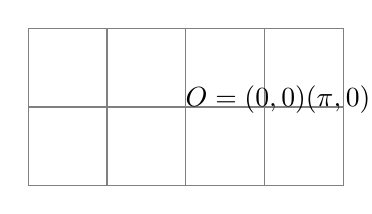
\begin{tikzpicture}
\draw[gray] (-2, -1) grid (2, 1);
\ShowPoint[color=teal, radius=2pt, type=pentagon*, opacity=.8, rotate=60]
    {(-1.5, 0); (2, .5)}[$O=(0, 0)$; $(\pi, 0)$]
    [above right=3pt and 0em, font=\small]
\end{tikzpicture}
\end{DocExample}


\begin{function}[added=2025-05-15]{\ShowIntersection}
  \begin{syntax}
    \cs{ShowIntersection}\oarg{key-val}\zarg{\meta{path-1}; \meta{path-2}}\marg{number}
  \end{syntax}
  此命令用于求解 \meta{path-1} 和 \meta{path-2} 的交点, 使用 ``;'' 进行分割; 然后将
  前 \meta{number} 个交点绘制出来. \meta{key-value} 对应 \cs{ShowPoint} 命令中的 \meta{key-value} 选项,
  即 \meta{ztikz/point}.
\end{function}
\begin{DocExample}*
\begin{tikzpicture}
\draw[gray] (-2, -1) grid (2, 1);
\draw[name path=line1] (-2, -.5) -- (2, .5);
\draw[name path=line2] (-1, 1) -- (1, -1);
\ShowIntersection[color=blue]{line1; line2}{1}
\end{tikzpicture}
\end{DocExample}



\begin{function}[added=2025-05-15]{\ShowAxis}
  \begin{syntax}
    \cs{ShowAxis}\oarg{key-value}\zarg{\meta{start}; \meta{end}}
  \end{syntax}
  此命令用于绘制坐标轴, \meta{start} 和 \meta{end} 分别表示坐标轴的起始点和结束点, 
  使用 ``;'' 进行分割, 坐标格式为 $(x, y)$. \meta{key-value} 为可选参数, 用于设置坐标轴样式.
\end{function}


\begin{keyval}[parent=ztikz/axis]
  {tickStart, tickEnd, axisRotate, mainStep, subStep, 
  tickLabelShift, mainTickLength, subTickLength,
  axisColor, mainTickColor, subTickColor, tickStyle,
  mainTickLabel, mainTickLabelColor, mainTickLabelPosition}
  \begin{syntax}
    tickStart       = \meta{浮点数}>\dval{-5}
    tickEnd         = \meta{浮点数}>\dval{5}
    axisRotate      = \meta{浮点数}>\dval{0}
    mainStep        = \meta{浮点数}>\dval{1}
    subStep         = \meta{浮点数}>\dval{0.1}
    tickLabelShift  = \meta{长度}>\dval{0pt}
    mainTickLength  = \meta{长度}>\dval{4pt}
    subTickLength   = \meta{长度}>\dval{2pt}
    axisColor       = \meta{颜色}>\dval{black}
    mainTickColor   = \meta{颜色}>\dval{black}
    subTickColor    = \meta{颜色}>\dval{black}
    tickStyle       = \meta{below|above|cross}>\dval{无}
    mainTickLabel   = \meta{字符串}>\dval{\cs{CurrentFp}}
    mainTickLabelColor    = \meta{颜色}>\dval{black}
    mainTickLabelPosition = \meta{\textbf{below}|above|cross}>\dval{below}
  \end{syntax}
  \meta{mainTickLabel} 主要用于自定义坐标标签的样式, \cs{CurrentFp} 表示当前刻度处
  的浮点数值. \meta{tickStyle} 会受到 \env{tikzpicture} 环境可选参数中的 \meta{rotate} 
  选项的影响.\par \textbf{注意}: 在使用 \cs{ShowAxis} 时若没有指定键 \meta{tickStyle} 的值,那
  么此时并不会绘制任何的刻度.
\end{keyval}



\begin{function}[added=2025-05-15]{\xAxis}
  \begin{syntax}
    \cs{xAxis}\oarg{start}\oarg{end}
  \end{syntax}
  此命令来自 \cs{ShowAxis}, 用于绘制 $x$ 轴; \meta{start} 和 \meta{end} 均为浮点数, 分别表示坐标轴的起始点和结束点.
\end{function}



\begin{function}[added=2025-05-15]{\yAxis}
  \begin{syntax}
    \cs{yAxis}\oarg{start}\oarg{end}
  \end{syntax}
  此命令来自 \cs{ShowAxis}, 用于绘制 $y$ 轴; \meta{start} 和 \meta{end} 均为浮点数, 分别表示坐标轴的起始点和结束点.
\end{function}
\begin{DocExample}*
\begin{tikzpicture}[>=Latex]
\yAxis[-1][1]
\ShowAxis{(-2, 0); (2, 0)}
\draw (-2, -1) grid (2, 1);
\end{tikzpicture}
\end{DocExample}



\begin{function}[added=2025-05-15]{\ShowGrid}
  \begin{syntax}
    \cs{ShowGrid}\oarg{draw-keyval}\zarg{\meta{start}; \meta{end}}
  \end{syntax}
  此命令用于绘制网格线, \meta{start} 和 \meta{end} 分别表示网格线的左下角和和右上角的坐标, 使用 ``;'' 进行分割, 
  坐标的格式为 $(x, y)$. \meta{key-value} 为可选参数, 用于设置网格线的样式;
\end{function}


\begin{function}[added=2025-05-15]{\Polygon}
  \begin{syntax}
    \cs{Polygon}\oarg{key-value}\marg{number}
  \end{syntax}
  此命令用于绘制正多边形, \meta{number} 表示多边形的边数, 其值必须为大于等于 3 的整数.
  \meta{key-value} 为可选参数, 用于设置多边形的样式;
\end{function}


\begin{keyval}[parent=ztikz/polygon]{
  radius, edgeColor, fillColor, fillOpacity, 
  rotate, shift, marker}
  \begin{syntax}
    radius      = \meta{浮点数}>\dval{1}
    edgeColor   = \meta{颜色}>\dval{black}
    fillColor   = \meta{颜色}>\dval{无}
    fillOpacity = \meta{浮点数}>\dval{0}
    rotate      = \meta{浮点数}>\dval{0}
    shift       = \meta{坐标}>\dval{(0, 0)}
    marker      = \meta{key-value}>\dval{无}
  \end{syntax}
  \meta{radius} 表示此正多边形外接圆的半径, 而非 \meta{marker} 的半径; \meta{shift}
  外围的 ``()'' 不能省略. \meta{marker} 对应 \meta{ztikz/point}. \meta{marker} 的设置
  请参见 \cref{fig:point-marker}.
\end{keyval}
\begin{DocExample}*
\begin{tikzpicture}
\ShowGrid[gray, thin]{(-2, -1); (2, 1)}
\Polygon[
  edgeColor=blue, shift={(1, 0)}, 
  marker={type=ball, color=green}
]{3}
\end{tikzpicture}
\end{DocExample}


\begin{function}[added=2025-05-15]{\StairsPlot}
  \begin{syntax}
    \cs{StairsPlot}[\meta{plot option}; \meta{jump option}]\oarg{draw-keyval}
    ~~~~~~~~~~~\oarg{key-value}\marg{file}
  \end{syntax}
  此命令用于绘制阶梯图, 绘图数据由 \meta{file} 指定; \meta{plot option} 用于设置阶梯图的绘制样式, 
  可选值有: \texttt{plot left, plot right, plot mid}; \meta{jump option} 用于设置阶梯图的跳跃样式,
  可选值有: \texttt{jump left, jump right, jump mid}; \meta{key-value} 对应 \meta{ztikz/point};
\end{function}
\begin{DocExample}*[@@]
\begin{tikzpicture}
\ShowGrid[step=1, color=gray]{(-4, -1); (4, 1)}
\StairsPlot[;jump-left][teal][type=ball, color=teal]{./sine.data}
\end{tikzpicture}
\end{DocExample}


\begin{function}[added=2025-05-15]{\StemPlot}
  \begin{syntax}
    \cs{StemPlot}\oarg{direction}\oarg{draw-keyval}
    ~~~~~~~~~\oarg{key-value}\marg{file}
  \end{syntax}
  此命令用于绘制火柴棍图, 绘图数据由 \meta{file} 指定; \meta{direction} 用于指定系列线段的方向, 
  可选值有: \texttt{x, y, o}, 分别表示垂直 $x$ 轴, 垂直 $y$ 轴, 以及指向坐标原点; \meta{key-value} 对应 \meta{ztikz/point}.
\end{function}
\begin{DocExample}*[@@]
\begin{tikzpicture}
\ShowGrid[step=1, color=gray]{(-4, -1); (4, 1)}
\StemPlot[x][red][type=*, color=red]{./sine.data}
\end{tikzpicture}
\end{DocExample}



\begin{function}[added=2025-05-15]{\BarPlot}
  \begin{syntax}
    \cs{BarPlot}\oarg{position}\oarg{draw-keyval}
    ~~~~~~~~\oarg{key-value}\marg{file}
  \end{syntax}
  此命令用于绘制条形图, 绘图数据由 \meta{file} 指定; \meta{position} 用于指定每个小矩形的位置以及宽度, 
  可选值有: \texttt{x, y, xc, yc}; \meta{key-value} 对应 \meta{ztikz/point}.
\end{function}
\begin{DocExample}*[@@]
\begin{tikzpicture}
\ShowGrid[step=1, color=gray]{(-4, -1); (4, 1)}
\BarPlot[x][red, pattern=north west lines, pattern color=red]{./sine.data}
\end{tikzpicture}
\end{DocExample}


\clearpage
\subsection{gnuplot 库}
需要说明的是: \TikZ{} 宏包内部已经提供了直接调用 gnuplot 程序的命令(需启用 \texttt{-shell-escape} 参数), 
其调用格式如下:
\def\exampleUR{}
\begin{DocExample}
  \draw/\oarg{key-value} plot\oarg{id} function\marg{function};/
\end{DocExample}

上述命令中 \meta{id} 用于区分不同的数据文件, 在 \texttt{\meta{file}.tex} 文件(不妨设文件名为 \meta{file})的根路径
下会产生两个文件:一个是 gnuplot 用于绘图的样式文件 \texttt{\meta{file}.\meta{id}.gnuplot}; 第二个是 gnuplot 产生的数据文件
\texttt{\meta{file}.\meta{id}.table}. 命令中的 \meta{function} 可用值请参见: \cref{tab:gnuplot-functions}. 

\TikZ{} 的内置命令也支持另外两种格式: ``\texttt{parametric}'', ``\texttt{raw gnuplot}'': 第一个参数表示
绘制参数方程, 第二个参数表示直接在文档中使用 gnuplot 的原始绘图命令(比如 ``\texttt{set samples 25; plot sin(x)}''). 
两者的调用格式如下:
\begin{DocExample}
  \draw/\oarg{key-value} plot [parametric,  \meta{id}]\marg{function};/
  \draw/\oarg{key-value} plot [raw gnuplot, \meta{id}]\marg{gnuplot code};/
\end{DocExample}
\resetExampleUR
\begin{DocExample}*
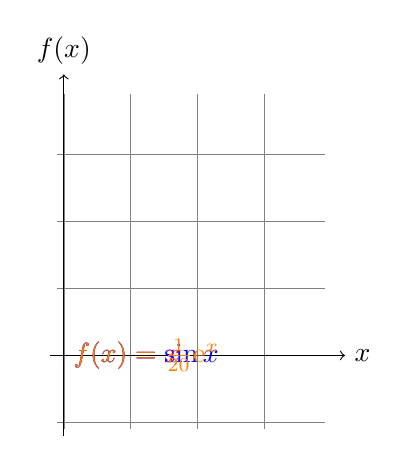
\begin{tikzpicture}[domain=0:4, scale=.85]
  \draw[very thin,color=gray] (-0.1,-1.1) grid (3.9,3.9);
  \draw[->] (-0.2,0) -- (4.2,0) node[right] {$x$};
  \draw[->] (0,-1.2) -- (0,4.2) node[above] {$f(x)$};
  \draw[color=red] plot[id=x] function{x} node[right] {$f(x)=x$};
  \draw[color=blue] plot[id=sin] function{sin(x)}node[right]{$f(x)=\sin x$};
  \draw[color=orange] plot[id=exp] function{0.05*exp(x)} node[right] {$f(x)=\frac{1}{20} \mathrm e^x$};
\end{tikzpicture}
\end{DocExample}

关于 \TikZ{} 中这部分原生绘图命令更加详细使用方法请参见\TikZ{} 官方文档中 \textsf{Section 22: Plots of Functions}.

但是为了 gnuplot 这一系列绘图命令的统一,\zTikZ{} 并没有采用上面的方式, 而是借用 \pkg{ztool} 宏包, 然后配合
预定义的绘图脚本去完成绘图任务. \zTikZ{} 中 \pkg{gnuplot} 库的绘图逻辑大致如下:
\begin{itemize}
  \item 首先通过 \pkg{ztool} 的 \cs{ztool_replace_file_line:nnn} 函数修改预定义的脚本;
  \item 然后通过命令行的 \texttt{-shell-escape} 参数去调用 gnuplot 运行修改后的脚本;
  \item 最后使用命令 \texttt{\cs{draw}\oarg{key-value} plot file \oarg{data};} 调用
    上一步生成的数据文件完成绘图.
\end{itemize}

不熟悉 gnuplot 的用户可阅读这份 7 页的快速入门指南: \href{http://www.gnuplot.info/docs_4.0/gpcard.pdf}{gnuplot card}.
\vskip1em
\noindent{\sffamily\color{red} NOTE: 调用此库后, 需在编译时启用 ``\texttt{-shell-escape}'' 参数.}


\begin{keyval}[parent=ztikz/2dplot]{domain, style, marker}
  \begin{syntax}
    domain  = \meta{浮点数:浮点数; 浮点数:浮点数}>\dval{\meta{不确定}}
    style   = \meta{draw-keyval}>\dval{black}
    marker  = \meta{key-value}>\dval{空}
  \end{syntax}
  \meta{maker} 中的 \meta{key-value} 对应 \meta{ztikz/point}. \meta{domain}
  二者之间使用 ``;'' 进行分割, 在不同的函数中 \meta{domain} 的意义不同: 
  在 \cs{Plot} 中用于设置自变量 $x$ 的范围; 在 \cs{ParamPlot} 和 \cs{PolarPlot} 中, 
  用于设置参数 $t$ 或极坐标系中角度 $\theta$ 的范围; 在 \cs{ContourPlot} 中, ``;'' 前后两个
  \meta{domain} 分别表示 $x$ 和 $y$ 的范围.
\end{keyval}


\begin{function}[added=2025-05-15]{\PlotPrecise}
  \begin{syntax}
    \cs{PlotPrecise}\marg{type}\marg{number}
    \cs{PlotPrecise}*\marg{type}\marg{number}
  \end{syntax}
  此命令用于设置 \pkg{gnuplot} 中一系列\textbf{二维}绘图函数对应的精度, \meta{type} 可选值有:
  ``\texttt{plot, param, polar, contour}'', 分别对应命令 \cs{Plot}, \cs{ParamPlot}, \cs{PolarPlot} 和 \cs{ContourPlot}
  的绘制精度. 含有 ``\texttt{*}'' 的命令会应用于对应绘图命令之后的所有实例, 没有 ``\texttt{*}'' 的命令仅会应用于之后的第一个绘图命令.
\end{function}



\begin{function}[added=2025-05-15]{\Plot}
  \begin{syntax}
    \cs{Plot}\oarg{key-value}\marg{function}
  \end{syntax}
  此命令用于绘制函数 $y=y(x)$, \meta{function} 为 gnuplot 中的函数表达式, 自变量为 ``\texttt{x}'';
  \meta{key-value} 用于设置绘图样式, 对应 \meta{ztikz/2dplot}. \meta{domain}
  默认为 \texttt{-5:5}. \textbf{注记:} 只需将 \meta{opacity} 置为 0, 即可实现散点图绘制.
\end{function}


\begin{function}[added=2025-05-15]{\ContourPlot}
  \begin{syntax}
    \cs{ContourPlot}\oarg{key-value}\marg{equation}
  \end{syntax}
  此命令用于绘制方程 $f(x, y)=c$, \meta{equation} 为 gnuplot 中的方程表达式, 变量为 ``\texttt{x, y}'', 
  且表达式中不需要书写 ``='' 符号; \meta{key-value} 用于设置绘图样式, 对应 \meta{ztikz/2dplot}. \meta{domain}
  默认为 ``\texttt{-5:5;*:*}'' (即自变量 $y$ 的范围自适应).\par 
  \noindent\textbf{注意}: 绘制 $x=c$ 这种垂直线段时, 可以使用此函数.
\end{function}



\begin{function}[added=2025-05-15]{\ParamPlot}
  \begin{syntax}
    \cs{ParamPlot}\oarg{key-value}\marg{equation}
  \end{syntax}
  此命令用于绘制参数方程 $x=x(t), y=y(t)$, \meta{equation} 为 gnuplot 中的方程表达式, 参数为 ``\texttt{t}'';
  \meta{key-value} 用于设置绘图样式, 对应 \meta{ztikz/2dplot}. \meta{domain}
  默认为 \texttt{0:2*pi}.
\end{function}



\begin{function}[added=2025-05-15]{\PolarPlot}
  \begin{syntax}
    \cs{PolarPlot}\oarg{key-value}\marg{equation}
  \end{syntax}
  此命令用于绘制极坐标方程 $\rho=\rho(t)$, \meta{equation} 为 gnuplot 中的方程表达式, 参数为 ``\texttt{t}'';
  \meta{key-value} 用于设置绘图样式, 对应 \meta{ztikz/2dplot}. \meta{domain}
  默认为 \texttt{0:2*pi}.
\end{function}


\begin{DocExample}*[@@]
\begin{tikzpicture}[>=Latex, scale=.4]
\ShowGrid{(-8, -8); (8, 8)}\ShowAxis{(0, -8); (0, 8)}\ShowAxis{(-8, 0); (8, 0)}
% draw functions/curves
\Plot[domain=-1:7.6, style=cyan] {-.9*x+7}
\ContourPlot[
  domain={-3:pi; -3:exp(1)}, style={red, thick}
]{x**2 + y**2 - 10}
% change plot precise
\PlotPrecise{plot}{1500}
\Plot[domain=-7:7.8]{3*sin(1/x)}
\Plot[domain=-1.5:7.5, style=green] {x*exp(-x)}
\ParamPlot[domain=0:2*pi, style=red]{7*sin(t), 4*cos(t)}
\end{tikzpicture}
\hskip.5em
\begin{tikzpicture}[>=Latex, scale=.4]
\ShowGrid{(-8, -8); (8, 8)}\ShowAxis{(0, -8); (0, 8)}\ShowAxis{(-8, 0); (8, 0)}
% draw functions/curves
\begin{scope}[xshift=4cm, yshift=-5cm]
  \PolarPlot[domain=0:10*pi, style=orange]{0.1*t}
\end{scope}
\begin{scope}[xshift=-4cm, yshift=5cm]
  \PolarPlot{2*(1-sin(t))}
\end{scope}
\end{tikzpicture}
\end{DocExample}

回顾上面给出的这个简单案例: 这个案例中我们使用了 \cs{Plot}, \cs{ParamPlot}, \cs{PolarPlot} 和 
\cs{ContourPlot} 四个命令; 同时也应用了 \cs{PlotPrecise} 命令, 它更改了 \cs{Plot} 命令的绘制精度.


\begin{keyval}[parent=ztikz/3dplot]{domain, pm3d, width, palette}
  \begin{syntax}
    domain  = \meta{浮点数:浮点数; 浮点数:浮点数}>\dval{-5:5; -5:5}
    pm3d    = \meta{\textbf{true}|false}>\dval{true}
    width   = \meta{长度}>\dval{0.75\string\linewidth}
    palette = \meta{字符串}>\dval*{rgbformulae~ 22,13,-31}
  \end{syntax}
  \meta{domain} 用于设置自变量 $x$ 和 $y$ 的取值范围, 二者之间使用 ``;'' 进行分割;
  \meta{pm3d} 用于控制是否启用曲面染色, 若 \meta{pm3d}\texttt{=false} 则此时进绘制曲面的
  一系列曲线; \meta{width} 用于设置该图片的宽度. 
\end{keyval}


\begin{function}[added=2025-05-15]{\Plotz}
  \begin{syntax}
    \cs{Plotz}\oarg{key-value}\marg{function}
  \end{syntax}
  此命令用户绘制普通的二维显式函数, \meta{function} 为 gnuplot 中的函数表达式;
  \meta{key-value} 用于设置绘图样式, 对应 \meta{ztikz/3dplot}. \textbf{注意}: 
  该命令不能在 \cs{tikzpicture} 环境中使用. 
\end{function}

下面这个案例展示了 \cs{Plotz} 命令的基本使用方法, 其中第一个案例内的 ``\texttt{x**2+y**2-2 with pm3d}'' 
为 gnuplot 所特有的语法, 详细信息请参见 gnuplot 手册.
\begin{DocExample}*
\Plotz[
  pm3d = false,
  width = .45\linewidth,
  domain = {-3:3; -3:3}
]{x**2+y**2-2 with pm3d, -x**2-y**2+8 with lines}
\hskip5em
\Plotz[
  pm3d, 
  width = .45\linewidth,
  domain = {-3:3; -3:3},
  palette = {cubehelix start 0 cycles -1. saturation 1}
]{x**2-y**2-2}
\end{DocExample}



\begin{function}[added=2025-05-15]{\currentTikzIndex}
  该命令表示当前 \env{tikzpicture} 环境的索引, 返回值为整数, 从 1 开始.
\end{function}


\begin{function}[added=2025-05-15]{\gnudata}
  \begin{syntax}
    \cs{gnudata}\oarg{index}
  \end{syntax}
  该命令会用引用当前 \env{tikzpicture} 环境中产生的绘图数据, 返回一个(数据)文件名, 从 1 开始.
  \meta{index} 接受一个整数, 表示当前环境中绘图数据的编号. 每一个已经绘制的函数都会在对应的文件夹
  下生成一个对应的数据文件,用户可以使用此数据文件进行后续的绘图操作.
\end{function}

\cmd{\gnudata} 的用法补充说明, 为后面区域填充案例做铺垫: 比如 \verb|\gnudata{2}|, 参数中
的 ``2'' 表示此数据是在当前 \env{tikzpicture} 环境中的第二个函数绘图数据; 所以在第一个 \env{tikzpicture} 环境中
它的返回值可能为 ``\texttt{./ztikz_output/gnuplot_data/gnu_data_1_2.table}''.

\begin{figure}[!htb]
  \centering
  
\includegraphics[width=.5\linewidth]{./support//pics/contour_data_bug.pdf}
  \caption{\cs{ContourPlot} Fill Issue}
  \label{fig:contour-fill-bug}
\end{figure}

\textbf{注意}: 由于技术原因,\cmd{\ContourPlot} 命令生成的数据暂时不可用于后续填充操作. 可考虑先将隐函数转化为
参数方程形式或极坐标形式, 再导出对应的数据. 如果你强行使用此类型数据,那么用户可能会得到类似 \cref{fig:contour-fill-bug} 
这样的不良输出.


\clearpage
\subsection{cache 库}
当用户加载 \pkg{cache} 库后, 随后在命令行中编译文档, 不妨设其名称为 \meta{file}; 那么用户会看到如下的日志输出:


\def\exampleUR{}
\begin{DocExample}
\write18 enabled.
entering extended mode
\end{DocExample}


编译结束后, 在你的项目文件夹下会生成一个名为 \file{ztikz_output} 的文件夹, 这个文件夹在你
第一次调用 \pkg{ztikz} 宏包时便会产生; 这个文件夹用于存放 \zTikZ{} 的缓存文件: 包括 \TikZ{} 
\pkg{external} 库的缓存结果, Python 脚本的缓存结果, WolframScript 脚本的缓存结果, 以及 gnuplot 的 
一系列缓存结果.

现在我们来说说这个文件夹的构成: 比如, 若用户运行了 \cmd{\Plot} 命令, 此时会在 \file{ztikz_output/tikz_data/} 
目录下生成了如 \cref{fig:zTikZ-directory} 中所示的 4 个文件:

\begin{figure}[!htb]
  \centering
  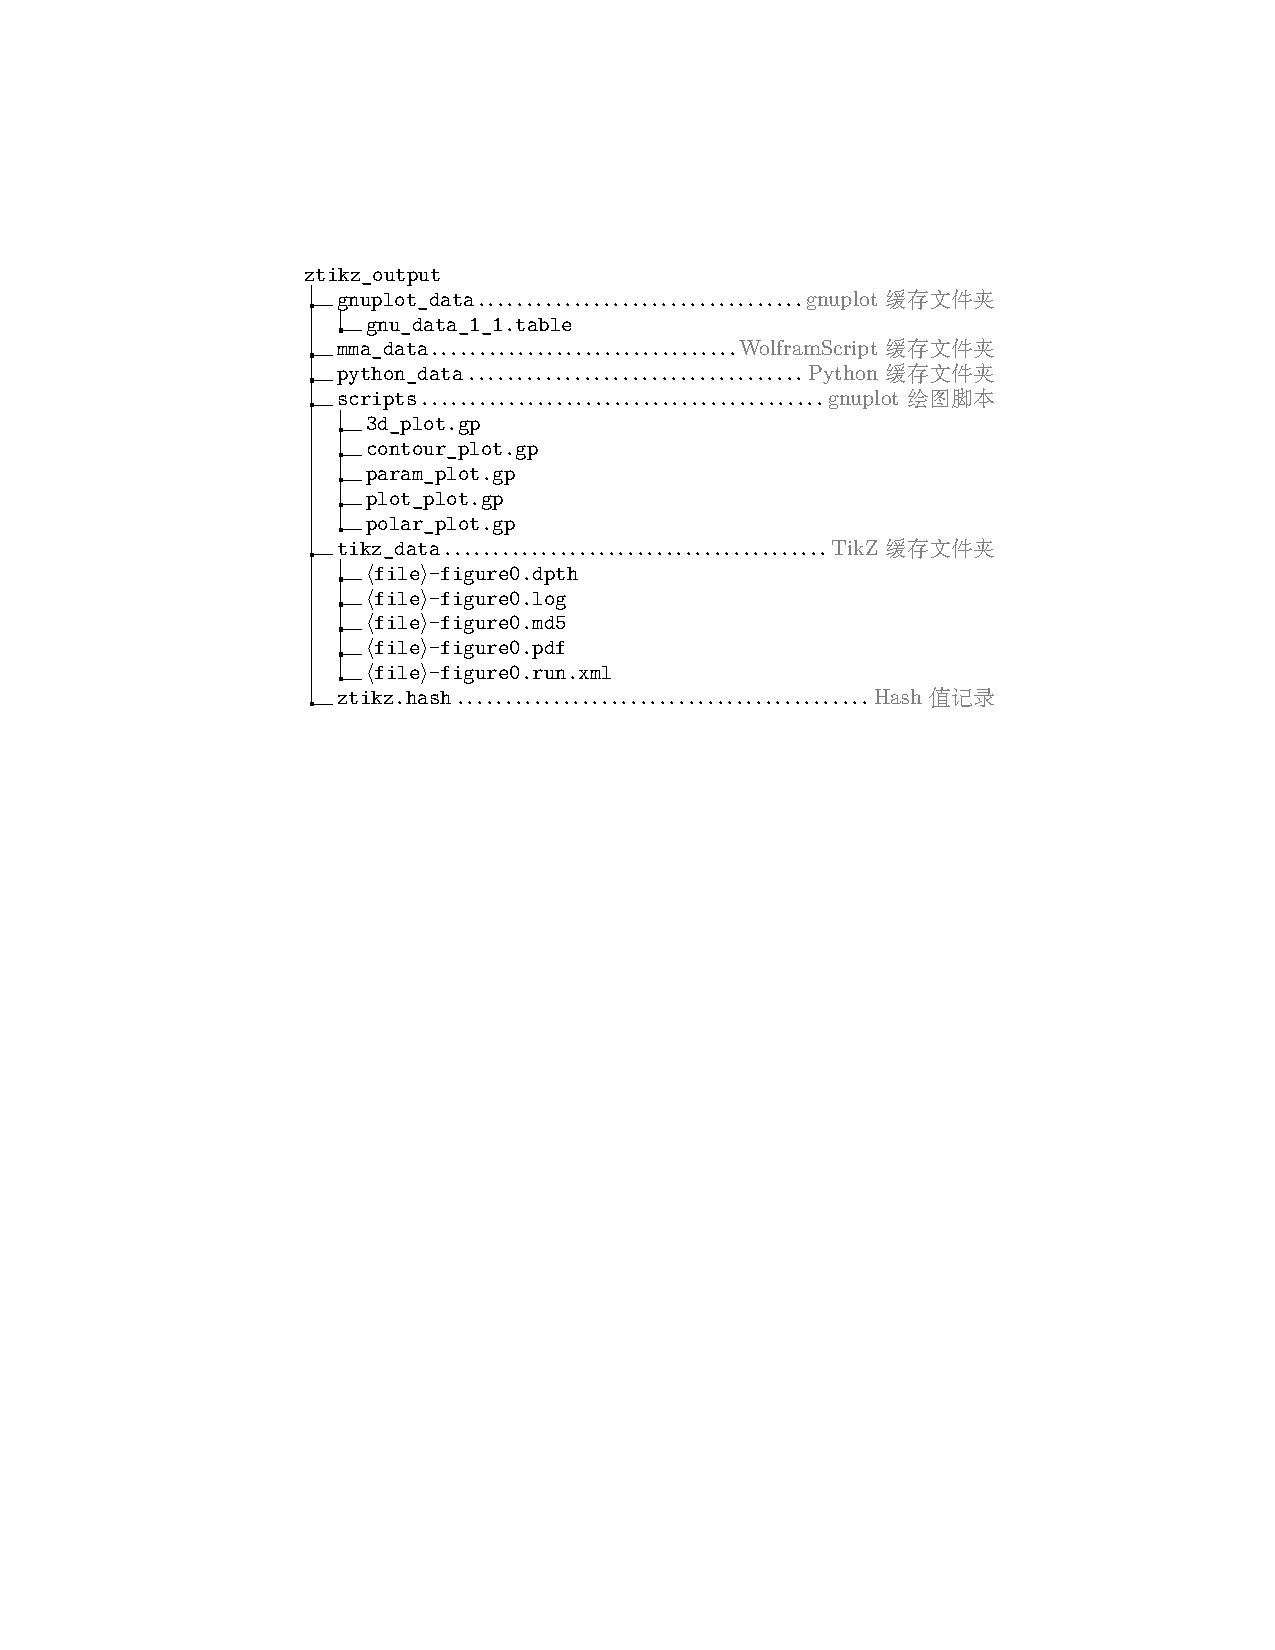
\includegraphics[width=.9\linewidth]{./support/pics/directory_tree_crop.pdf}
  \caption{\zTikZ{} 缓存目录结构示意图}
  \label{fig:zTikZ-directory}
\end{figure}

\file{tikz_data} 中的 \texttt{\meta{file}-figure0.pdf} 为 \env{tikzpicture} 环境缓存的 PDF 文件; 
此时在对应的 \texttt{\meta{file}.md5} 文件中可以看到如下内容:


\begin{DocExample}
\def \tikzexternallastkey {AE7F2539E81C96848ADCCEE3994993D1}%
\end{DocExample}
\resetExampleUR


上述命令保存了此 \env{tikzpicture} 环境中代码的 Hash 值, 当我们改变 \env{tikzpicture} 环境中
的代码时, 这个 Hash 值就会改变,从而 \TikZ{} 就会再次运行此环境, 重新生成图片. 这便是 \TikZ{} 的
\pkg{external} 库所提供的缓存功能的大致描述. \zTikZ{} 中的 Cache 机制和此原理是十分类似的.


\begin{function}[added=2025-05-15]{\ztikzHashClean}
  此命令用于不接受任何的参数, 用于清除之前缓存的所有 Hash 值.
\end{function}


\begin{function}[added=2025-05-15]{\ztikzHashCurrent}
  \begin{syntax}
    \cs{ztikzHashCurrent}*
    \cs{ztikzHashCurrent}\oarg{separator}
  \end{syntax}
  此命令主要用于调试或与命令 \cs{ztikzHashchgNorun} 配合使用; \texttt{\cs{ztikzHashCurrent}*} 将输出最近的一次 Hash 值计算结果;
  \cs{ztikzHashCurrent}\oarg{separator} 用于输出截至目前位置所有缓存的 Hash 值, 以 \meta{separator} 分隔输出到 PDF.
  \meta{separator} 默认为 ``\texttt{,}''.
\end{function}


\begin{function}[added=2025-05-15]{\ztikzHashchgNorun}
  \begin{syntax}
    \cs{ztikzHashchgNorun}\oarg{type}\marg{hash}
  \end{syntax}
  此命令用于决定 Hash 值改变后是否再次调用外部程序, 作用于它之后的第一个具有 cache 机制的环境或命令; 建议配合 \cs{ztikzHashCurrent}
  使用. \meta{type} 表示上一次缓存内容的文件类型, 默认为 ``\texttt{txt}'', 可选值有: ``\texttt{txt}, \texttt{pdf}'' 等. 
  \meta{hash} 为该环境或命令改变之前的 Hash 值, 且后续 \cs{wolframResult} 或 \cs{wolframOuputFile} 命令都将引用该命令或环境之
  前 Hash 值为 \meta{hash} 时的结果. \textbf{注意}: 目前该命令仅对 \pkg{wolfram} 库中的命令或环境有效.
\end{function}


\clearpage
\subsection{python 库}
\pkg{python} 库主要用于和 Python 交互, 其使用方法和 \pkg{gnuplot} 库类似. \pkg{python} 
库中主要提供了图片绘制与计算接口, 其中计算接口包含数值计算与符号计算.

除去 \ztikz{} 提供的 Python 绘图功能外,我们需要着重说明 \zTikZ{} 提供的的浮点数计算功能: 
\zTikZ{} 在调用此库时默认导入 Python 的 \pkg{numpy}, \pkg{sympy}, \pkg{scipy} 三个包; 此外, 用户在
使用 \pkg{numpy} 中的函数时不用再加以前缀, 比如求解 $\sin(2.345)$ 时, 直接使用 \verb|\py{sin(2.345)}| 即可, 
不必写为 \verb|\py{np.sin(2.345)}| 之类的格式了. 对于其它 Python 库中的函数, 使用方法同理.

\vskip1em
\noindent{\sffamily\color{red} NOTE: 调用此库后, 需在编译时启用 ``\texttt{-shell-escape}'' 参数.}



\begin{function}[added=2025-05-15]{\py}
  \begin{syntax}
    \cs{py}\oarg{\textbf{raw}|str}\marg{code}
  \end{syntax}
  此命令会调用 Python 进行浮点数运算, \meta{code} 为合法的 Python 表达式; 这部分的结果并不会被缓存,也就是说每次编译此
  文档时,Python 都会重新计算此部分的结果. 用户可以把 \cmd{\py} 命令嵌套到自己定义的宏命令中. \par
  \textbf{注意}: \meta{raw} 会将返回的结果按照 \TeX{} 原始的 catcode 进行 tokenize; \meta{str} 则是将返回的
  结果处理为 string.
\end{function}
\begin{DocExample}*
\newcommand{\pypow}[1]{\py{#1}}
\newcommand{\pyreverse}[1]{\py{'#1'[::-1]}}
\newcommand{\pyuppercase}[1]{\py{'#1'.upper()}}
\begin{itemize}
  \item Power Calculation: $2^{10} = \pypow{2**10}$
  \item Reverse a string using Python: \pyreverse{Hello-LaTeX}
  \item Uppercase a string: \pyuppercase{hello-latex}
  \item Modulus: $102 = \py{mod(102, 8)} \mod 8$
  \item Return string Options: \py[str]{'$$'+str(2**10)+'$$'}
\end{itemize}
\end{DocExample}


\begin{function}[added=2025-05-15]{\sympy}
  \begin{syntax}
    \cs{sympy}\marg{expression}
  \end{syntax}
  此命令主要用于调用 Python 的 \pkg{sympy} 库进行符号计算, \meta{expression} 为符号表达式. \zTikZ{} 对此
  命令提供了 cache 机制. \pkg{python} 库中预定义了一系列的符号变量, 包括: \texttt{x, y, z, u, v, t}, 这些预定义变量无需用户再次声明.
  \par \textbf{注意}: 默认的情况下, 此命令的返回结果中包含: \verb|^, _| 等特殊字符, 所以请将此命令置于数学环境中.
\end{function}
\begin{DocExample}*
\[
  \int x^8 + \cos(7x) + 6t\,\mathrm{d}x  
    = \sympy{integrate( x**8 + cos(7*x) + 6*t, x )}    
\]
\[
  \mathrm{eig}(\begin{bmatrix}1 & 2\\2 & 2\end{bmatrix})
    = \sympy{Matrix([[1, 2], [2, 2]]).eigenvals()}    
\]
\end{DocExample}


\begin{function}[added=2025-05-15]{pyfig}
  \begin{syntax}
    \cs{begin}\zarg{pyfig}\oarg{spec}\marg{file} 
    ~~~~\meta{plot code} 
    \cs{end}\zarg{pyfig}
  \end{syntax}
  此环境用于调用 Python 进行绘图, 具有缓存机制; \meta{spec} 用于设置图片的的排版参数, 默认为 \verb|width=.75\linewidth|;
  \meta{file} 用于设置当前代码片段对应的文件名. 该命令返回的结果为: \texttt{\cs{includegraphics}\oarg{spec}\marg{file}.pdf},
  用户可以将此命令嵌入 \env{figure} 或 \env{table} 等浮动体环境中. \par 
  \textbf{注意}: 针对不同的 \env{pyfig} 环境请使用不同的 \meta{file} 值; 用户不需要在代码末尾添加 \verb|plt.savefig()| 命令,
  \ztikz{} 会自动处理相关的问题. 代码在抄录过程中会保留用户的缩进格式, 从行首开始抄录, 所以请不要添加多余的行首缩进.  
\end{function}
\begin{DocExample}*
\begin{pyfig}[width=.5\linewidth]{pycode.py}
import matplotlib
matplotlib.use('Agg')
from matplotlib import pyplot as plt
import numpy as np
x = np.linspace(0, 2*np.pi, num = 80)
y = np.sin(x)*np.cos(x)+.2
plt.plot(x, y)
\end{pyfig}
\end{DocExample}


\begin{function}[added=2025-05-15]{pycode}
  \begin{syntax}
  \cs{begin}\zarg{pycode}\marg{file} 
  ~~~~\meta{any python code} 
  \cs{end}\zarg{pycode}
  \end{syntax}
  此环境会将其内的代码抄录到 \meta{file} 中, 然后 \ztikz{} 会自动调用 Python 执行该文件, 但其不会返回任何结果;
  该环境的执行结果保存在文件 \texttt{\meta{file}.out} 中, 用户需要使用 \cs{input} 命令自行导入. 此环境同样具有
  cache 机制. \textbf{注意}: 代码在抄录过程中会保留用户的缩进格式, 从行首开始抄录, 所以不要过度使用缩进.
\end{function}
下面是一个关于 \env{pycode} 环境的简单使用示例, \file{table.py} 对应的内容请参见 \cref{imple:code-data}.
\begin{DocExample}*[@@]
\input{./table.py}
\end{DocExample}



\clearpage
\subsection{wolfram 库}
用户需注意 WolframScript 脚本中注释的写法, 不是 ``\verb|(* something*)|'', 而是 ``\verb|(* something *)|'',
即注释内容不能够紧挨 ``\verb|*|'', 否则可能会造成 WolframScript 的解析错误.

由于 WolframScript 的限制, 脚本的后缀只能为: ``\texttt{.wls}'', 否则 WolframScript
会无法识别此脚本(也就不会去执行此脚本了). 

\textbf{注记}: \ztikz{} 的 \pkg{wolfram} 库可以在 Windwos/Linux/MacOs 三大平台上使用, 并且可以在
对应环境的源码中键入 ``\verb|\, #, $, _, ^, &|'' 等特殊字符, 极大的弥补了 \href{https://github.com/stevenliuyi/latex-alpha2}{\pkg{latexalpha2}} 的不足.

\vskip1em
\noindent{\sffamily\color{red} NOTE: 调用此库后, 需在编译时启用 ``\texttt{-shell-escape}'' 参数.}

\begin{function}[added=2025-05-15]{\wolframResult}
  \begin{syntax}
    \cs{wolframResult}\oarg{separator}
    \cs{wolframResult}*\oarg{index}
  \end{syntax}
  此命令用于引用前一次 WolframScript 的计算结果, \texttt{\cs{wolframResult}\oarg{separator}} 
  表示使用 \meta{separator} 进行分隔, 然后引用全部计算结果; \texttt{\cs{wolframResult}*\oarg{index}}
  仅引用部分计算结果, \meta{index} 为整数或整数表达式, 默认为 1.
\end{function}


\begin{function}[added=2025-05-15]{\wolframOuputFile}
  此命令会返回 WolframScript 上次运行结果对应的文件名; 此命令在引用一些图片结果时是十分方便的.
  此命令比之 \cs{wolframResult} 更加的灵活, 前者调用上一次的文本文件, 后者仅返回上次 WolframScript 调用
  产生的文件名.
\end{function}


\begin{function}[added=2025-05-15]{\wolfram}
  \begin{syntax}
    \cs{wolfram}\marg{code}
    \cs{wolfram}*\marg{code}
  \end{syntax}
  此命令用于调用 WolframScript 中的进行计算, 具有缓存机制; \meta{code} 为合法的 WolframScript 代码;
  默认返回 \LaTeX{} 格式的代码, 含有 ``\texttt{*}'' 的命令返回的结果为普通的字符串(catcode 并没有改变).
\end{function}
\begin{DocExample}*
\wolfram{LaplaceTransform[t^4 Sin[3*t], t, s]}
\[
  \mathcal{L}(t^4\sin(3t)) = \wolframResult
\]
\end{DocExample}


\begin{function}[added=2025-05-18]{\wolframTex}
  \begin{syntax}
    \cs{wolframTex}\marg{Tex code}
  \end{syntax}
  此命令和上述的 \cs{wolfram} 命令类似, 不同的是, 此命令会将 \meta{Tex code} 中的所有内容转化为对应的
  Mathematica 代码, 返回的结果为 \LaTeX{} 代码. \par
  \vskip1em
  \noindent{\sffamily\color{red}NOTE: 由于此命令的实现原理较为复杂与特殊, 所以 \meta{Tex code} 中不能
  包含 ``\verb|$|'' 符号, 否则会出现解析错误.} 
\end{function}
\begin{DocExample}*
\wolframTex{\int_a^b\sin(x)\,dx}
\[
  \int_a^b \sin(x)\,dx = \wolframResult
\]
\end{DocExample}


\begin{function}[added=2025-05-15]{\wolframSolve}
  \begin{syntax}
    \cs{wolframSolve}\oarg{key-value}\marg{equation}
    \cs{wolframSolve}*\marg{full code}
  \end{syntax}
  此命令用于调用 WolframScript 中的进行方程的求解, 具有缓存机制; \meta{equation} 表示方程的表达式;
  \meta{key-value} 用于设置求解的自变量与定义域; \meta{full code} 为完整的方程表达式, 包含自变量, 定义域; 
\end{function}

\begin{keyval}[parent=ztikz/wolfram/solve]{domain, var}
  \begin{syntax}
    domain = \meta{定义域}>\dval{空}
    var    = \meta{变量}>\dval{空}
  \end{syntax}
  \meta{domain} 用于设置方程求解的``范围'', 比如 \texttt{\meta{domain}=Integers} 表示在整数范围内求解;
  \meta{var} 用于设置求解的自变量, 比如 \texttt{\meta{var}=x} 表示求解 $x$ 对应的表达式(等式左边为 $x$);
\end{keyval}

\begin{DocExample}*
\wolframSolve[var={x, y}]{a x + y == 8 && b x - y == 1}
\begin{align}
  &  \wolframResult \\
  &  \wolframResult[||] \\
  &  \wolframResult* \\
  &  \wolframResult*[3-1]
\end{align}
\wolframSolve[
  var={x, y}, domain=Integers
]{x^2 + 2 y^3 == 3681 && x > 0 && y > 0}
\begin{align}
  \wolframResult
\end{align}
\end{DocExample}


\begin{function}[added=2025-05-15]{\wolframDSolve}
  \begin{syntax}
    \cs{wolframDSolve}\oarg{key-value}\marg{equation}
    \cs{wolframDSolve}*\marg{full code}
  \end{syntax}
  此命令用于调用 WolframScript 中的进行微分方程的求解, 具有缓存机制; \meta{equation} 表示方程的表达式;
  \meta{key-value} 用于设置求解的自变量与定义域; \meta{full code} 为完整的微分方程表达式, 包含自变量, 因变量; 
\end{function}


\begin{keyval}[parent=ztikz/wolfram/dsolve]{depend, independ}
  \begin{syntax}
    depend    = \meta{因变量}>\dval{y[x]}
    independ  = \meta{自变量}>\dval{x}
  \end{syntax}
  \meta{depend} 用于指定该微分方程的因变量, 比如 \texttt{\meta{depend}=y[x]} 表示 $y$ 是 $x$ 的函数;
  \meta{independ} 用于指定该微分方程的自变量, 比如 \texttt{\meta{independ}=x} 表示 $x$ 是自变量;
\end{keyval}
\begin{DocExample}*
\wolframDSolve{y'[x] + y[x] == a*Sin[x], y[0] == 1}
\begin{align}
  &\wolframResult
\end{align}
\wolframDSolve[depend={y[x], z[x]}]{y'[x] == Exp[z[x]] + 1, z'[x] == y[x] - x}
\begin{align}\left\{\begin{aligned}
  &\wolframResult[\\&]
\end{aligned}\right.\end{align}
\end{DocExample}



\begin{function}[added=2025-05-15]{wolframGraphics}
  \begin{syntax}
    \cs{begin}\zarg{wolframGraphics}\oarg{spec} 
    ~~~~~\meta{plot code}
    \cs{end}\zarg{wolframGraphics}
  \end{syntax}
  此环境用于调用 WolframScript 进行绘图, 具有缓存机制; \meta{spec} 用于设置图片的的排版参数, 默认为空,
  此时该环境不会返回任何的结果, 可以通过 \cs{wolframOuputFile} 调用其产生的文件; 
  \meta{spec} 可以设置值, 对应图片的排版参数, 比如 \verb|width=10em|; 若 \meta{spec} 非空, 则该环境会
  返回: \texttt{\cs{includegraphics}\oarg{spec}\zarg{\meta{path}/\meta{HASH}.pdf}}, 其中 \meta{HASH} 
  为当前 \env{wolframGraphics} 环境中代码的 Hash 值, \meta{path} 为 WolframScript 缓存文件夹对应的目录.\par
  \vskip.5em
  \noindent{\sffamily\color{red} NOTE: \meta{plot code} 中最后得到的图片名称必须为 ``\texttt{FIGURE}'', 否则会报错.}
\end{function}
\begin{DocExample}*
\begin{wolframGraphics}
  FIGURE=Plot[Sin[x], {x, -Pi, Pi}]
\end{wolframGraphics}

\includegraphics[width=.5\linewidth]{\wolframOuputFile}
\end{DocExample}





\clearpage
\subsection{l3draw 库}
\zTikZ{} 基于 \pkg{l3draw} 宏包封装了一个 \pkg{l3draw} 库, 此库主要用于完成一些比较简单的绘图需求. 
在普通用户层面: \pkg{l3zdraw} 库提供了 \cs{zrule} 和 \cs{zplot} 两个命令, 前者用于绘制渐变矩形,
后者用于绘制函数, 同样也支持渐变; \ztikz{} 也对 \pkg{l3draw} 提供的绘图环境与命令进行了简单的封装, 
目前不是很完善, 且不稳定, 不推荐普通用户使用.


\begin{function}[added=2025-05-15]{\zdrawSetUnit}
  \begin{syntax}
    \cs{zdrawSetUnit}\oarg{unit}
  \end{syntax}
  此命令用于设置当前绘图的单位, 例如 \meta{unit} 可以取值为 ``\texttt{cm}''.
\end{function}


\begin{function}[added=2025-05-15]{\zdrawSetPathWidth}
  \begin{syntax}
    \cs{zdrawSetPathWidth}\oarg{width}
  \end{syntax}
  此命令用于设置当前绘图的线宽, 例如 \meta{width} 可以取值为 ``\texttt{0.5pt}'';
  \pkg{l3draw} 中默认的线径为 \texttt{0.4pt}.
\end{function}


\begin{function}[added=2025-05-15]{\zrule}
  \begin{syntax}
    \cs{zrule}\oarg{key-value}
  \end{syntax}
  此命令用于绘制渐变矩形, \meta{key-value} 用于设置渐变矩形的属性.
\end{function}

\begin{keyval}[parent=ztikz/zdraw/zrule]{width, height, startColor, endColor, step}
  \begin{syntax}
    width      = \meta{浮点数}>\dval{1}
    height     = \meta{浮点数}>\dval{1}
    startColor = \meta{颜色}>\dval{red}
    endColor   = \meta{颜色}>\dval{blue}
    step       = \meta{浮点数}>\dval{0.25}
  \end{syntax}
  \meta{width} 和 \meta{height} 用于设置渐变矩形的宽度和高度; 
  \meta{startColor} 和 \meta{endColor} 用于设置渐变矩形的起始颜色和结束颜色;
  \meta{step} 用于控制渐变精度.
\end{keyval}
\begin{DocExample}*
\zrule[width=10, startColor=red, step=1]
\end{DocExample}


\begin{function}[added=2025-05-15]{\zplot}
  \begin{syntax}
    \cs{zplot}\oarg{key-value}\marg{function}
  \end{syntax}
  此命令用于绘制函数, 水平方向和垂直方向的渐变, \meta{key-value} 用于设置函数的属性;
  \meta{function} 为合法的函数表达式. \par
  \vskip2em
  \noindent{\sffamily\color{red}NOTE: 目前 \cs{zplot} 命令不太稳定, 在部分情况下可能会报错, 用户应该谨慎使用该命令.}  
\end{function}


\begin{keyval}[parent=ztikz/zdraw/zplot]{action, domain, range, startColor, endColor, axis}
  \begin{syntax}
    action = \meta{\textbf{draw}|stroke|fill|clip|shade}>\dval{draw}
    domain = \meta{浮点数, 浮点数, 浮点数}>\dval{-5, 0.1, 5}
    range  = \meta{浮点数, 浮点数}>\dval{-5, 5}
    startColor = \meta{颜色}>\dval{black}
    endColor   = \meta{颜色}>\dval{white}
    axis       = \meta{x|\textbf{y}}
  \end{syntax}
  \meta{action} 用于控制绘制的行为; \meta{domain} 用于设置函数的自变量范围, 其中第一个浮点数为起始值, 
  第二个浮点数为步长, 第三个浮点数为结束值; \meta{range} 用于设置 $y$ 轴范围, 在 \meta{action}\texttt{=shade}
  时比较有用; \meta{startColor} 和 \meta{endColor} 用于设置函数的起始颜色和结束颜色; \meta{axis} 用于设置 
  渐变方式, `\texttt{x}' 对应水平渐变, `\texttt{y}' 对应垂直渐变.
\end{keyval}
\begin{DocExample}
\zplot[
  domain={0, 0.02*\c_pi_fp, 2*\c_pi_fp}, 
  action=shade, startColor=blue,
  endColor=green, axis=x]{sin(x)}
\zplot[
  domain={0, 0.02*\c_pi_fp, 2*\c_pi_fp}, 
  action=shade, startColor=blue,
  endColor=green, axis=y]{sin(x)}
\end{DocExample}


\begin{function}[added=2025-05-15]{Zdraw}
  \begin{syntax}
    \cs{begin}\zarg{zdraw} \meta{l3draw code} \cs{end}\zarg{zdraw}
  \end{syntax}
  此环境为 \cs{draw_begin:} 和 \cs{draw_end:} 的封装.
\end{function}


\begin{function}[added=2025-05-15]{Zgroup}
  \begin{syntax}
    \cs{begin}\zarg{zgroup} \meta{l3draw code} \cs{end}\zarg{zgroup}
  \end{syntax}
  此环境为 \cs{draw_path_scope_begin:} 和 \cs{draw_path_scope_end:} 的封装.
\end{function}


\begin{function}[added=2025-05-15]{\zmoveto, \zlineto}
  \begin{syntax}
    \cs{zmoveto}\marg{coordinate}
    \cs{zlineto}\marg{coordinate}
  \end{syntax}
  这两个命令用于移动当前画笔的坐标, \meta{coordinate} 为 \pkg{l3draw} 中合法的坐标表达式.
  比如 ``\texttt{1mm, 2cm+3em}''.
\end{function}


\begin{function}[added=2025-05-15]{\zscolor, \zfcolor}
  \begin{syntax}
    \cs{zmoveto}\marg{l3color}
    \cs{zlineto}\marg{l3color}
  \end{syntax}
  这两个命令用于移动当前画笔的坐标, \meta{l3color} 为 \pkg{l3draw} 中合法的颜色表达式;
  \ztikz{} 对常见的颜色预定义了其对应的 l3color 变量, 一些常见的颜色, 用户可以直接使用.
\end{function}


\begin{function}[added=2025-05-15]{\zxvec, \zyvec}
  \begin{syntax}
    \cs{zxvec}\marg{coordinate}
    \cs{zyvec}\marg{coordinate}
  \end{syntax}
  这两个命令用于设置当前坐标系的 $x$ 轴和 $y$ 轴的单位向量, \meta{coordinate} 为合法的坐标表达式;
  比如 ``\texttt{1mm, 2cm+3em}''.
\end{function}


\begin{function}[added=2025-05-15]{\zpolar, \zcoor}
  \begin{syntax}
    \cs{zpolar}\marg{radius}\marg{angle}
    \cs{zcoor}\marg{x-scale}\marg{y-scale}
  \end{syntax}
  \cs{zpolar} 命令按照极坐标的方式获取点的坐标:\meta{radius} 为合法的长度, 如 ``\texttt{2em}''; \meta{angle} 为浮点数; 
  \cs{zcoor} 命令按照直角坐标的方式获取点的坐标: \meta{x-scale} 为浮点数, \meta{y-scale} 为浮点数; 此命令获取的最终坐标
  还取决于 $x$ 和 $y$ 方向两个基向量的影响, (\meta{x-scale}, \meta{y-scale}) 也就是所谓的在基 \texttt{\{\cs{svec}, \cs{yvec}\}} 
  下的坐标.
\end{function}


\begin{function}[added=2025-05-15]{\zrect, \zcirc}
  \begin{syntax}
    \cs{zrect}\marg{coordinate}\marg{coordinate}
    \cs{zcirc}\marg{center}\marg{radius}
  \end{syntax}
  前者用于绘制矩形, 两个坐标点分别为矩形的左下角和右上角; 后者用于绘制圆形, \meta{center} 为圆心坐标, \meta{radius} 为半径;
  \meta{coordinate} 和 \meta{center} 均为合法的坐标表达式, 比如 ``\texttt{1mm, 2cm+3em}''.
\end{function}


\begin{function}[added=2025-05-15]{\znewtext, \zsethtext, \zsetvtext, \zscaletext, \zputtext}
  \begin{syntax}
    \cs{znewtext}\meta{coffin}
    \cs{zsethtext}\meta{coffin}\marg{content}
    \cs{zsetvtext}\meta{coffin}\marg{width}\marg{content}
    \cs{zscaletext}\meta{coffin}\marg{x-scale}\marg{y-scale}
    \cs{zputtext}\meta{coffin}\marg{hpole}\marg{vpole}\marg{point}
  \end{syntax}
  这系列命令用于在 \pkg{l3draw} 中创建, 变换与放置文本.
\end{function}


\begin{function}[added=2025-05-15]{\zbg, \zeg}
  这两个命令为 \cs{draw_path_scope_begin:} 和 \cs{draw_path_scope_end:} 的封装.
\end{function}



\begin{function}[added=2025-05-15]{\zcapbutt, \zcaproun, \zcaprect, \zclosepath}
  这系列命令用于设置线段之间的连接方式.
\end{function}


\begin{function}[added=2025-05-15]{\zshift, \zxscale, \zyscale, \ztrans}
  \begin{syntax}
    \cs{zshift}\marg{vector}
    \cs{zxscale}\marg{x-scale}
    \cs{zyscale}\marg{y-scale}
    \cs{ztrans}\marg{a}\marg{b}\marg{b}\marg{d}
  \end{syntax}
  这一系列的命令用于对坐标轴进行仿射变换, \cs{ztrans} 对应的仿射变换矩阵为:
  \[\begin{bmatrix}
    a & c\\
    b & d
  \end{bmatrix}\]
\end{function}


\begin{function}[added=2025-05-15]{\usepath}
  \begin{syntax}
    \cs{usepath}\marg{style}
  \end{syntax}
  此命令用于显示最终的路径, \meta{style} 的可选值有: ``\texttt{draw, stroke, fill, clip}''.
\end{function}


\clearpage
\section{附录}
\subsection{gnuplot Support Functions}
我们在这里补充说明 gnuplot 中内建的函数: Arguments to math functions in gnuplot can be integer, real, or 
complex unless otherwise noted. Functions that accept or return angles (e.g. $\sin(x)$) treat angle values as radians, 
but this may be changed to degrees using the command set angles.
(摘录自: \href{http://www.bersch.net/gnuplot-doc/expressions.html#expressions-functions-floor}{gnuplot support functions})

\begin{center}
  \begin{longtable}{lll}
    \caption{\textbf{gnuplot math library functions}}\\
    \toprule
    \textbf{Function} & \textbf{Arguments} & \textbf{Returns} \\
    \midrule
    \(\text{abs}(x)\) & any & $|x|$, absolute value of $x$; same type \\
    \(\text{abs}(x)\) & complex & length of $x$, $\sqrt{\text{Re}(x)^2 + \text{Im}(x)^2}$ \\
    \(\text{acos}(x)\) & any & $\cos^{-1} x$ (inverse cosine) \\
    \(\text{acosh}(x)\) & any & $\cosh^{-1} x$ (inverse hyperbolic cosine) in radians \\
    \(\text{airy}(x)\) & any & Airy function $\text{Ai}(x)$ \\
    \(\text{arg}(x)\) & complex & the phase of $x$ \\
    \(\text{asin}(x)\) & any & $\sin^{-1} x$ (inverse sine) \\
    \(\text{asinh}(x)\) & any & $\sinh^{-1} x$ (inverse hyperbolic sine) in radians \\
    \(\text{atan}(x)\) & any & $\tan^{-1} x$ (inverse tangent) \\
    \(\text{atan2}(y,x)\) & int or real & $\tan^{-1}(y/x)$ (inverse tangent) \\
    \(\text{atanh}(x)\) & any & $\tanh^{-1} x$ (inverse hyperbolic tangent) in radians \\
    \(\text{EllipticK}(k)\) & real  $k$ in $(-1:1)$ & $K(k)$ complete elliptic integral of the first kind \\
    \(\text{EllipticE}(k)\) & real  $k$ in $[-1:1]$ & $E(k)$ complete elliptic integral of the second kind \\
    \(\text{EllipticPi}(n,k)\) & real $n,|k|<1$ & $\Pi(n,k)$ complete elliptic integral of the third kind \\
    \(\text{besj0}(x)\) & int or real & $J_0$ Bessel function of $x$, in radians \\
    \(\text{besj1}(x)\) & int or real & $J_1$ Bessel function of $x$, in radians \\
    \(\text{besy0}(x)\) & int or real & $Y_0$ Bessel function of $x$, in radians \\
    \(\text{besy1}(x)\) & int or real & $Y_1$ Bessel function of $x$, in radians \\
    \(\text{ceil}(x)\) & any & $\lceil x \rceil$, smallest integer not less than $x$ (real part) \\
    \(\text{cos}(x)\) & radians & $\cos x$, cosine of $x$ \\
    \(\text{cosh}(x)\) & any & $\cosh x$, hyperbolic cosine of $x$ in radians \\
    \(\text{erf}(x)\) & any & $\text{erf}(\text{Re}(x))$, error function of $\text{Re}(x)$ \\
    \(\text{erfc}(x)\) & any & $\text{erfc}(\text{Re}(x))$, $1.0 - $ error function of $\text{Re}(x)$ \\
    \(\text{exp}(x)\) & any & $e^x$, exponential function of $x$ \\
    \(\text{expint}(n,x)\) & any & $E_n(x)$, exponential integral function of $x$ \\
    \(\text{floor}(x)\) & any & $\lfloor x \rfloor$, largest integer not greater than $x$ (real part) \\
    \(\text{gamma}(x)\) & any & $\Gamma(\text{Re}(x))$, gamma function of $\text{Re}(x)$ \\
    \(\text{ibeta}(p,q,x)\) & any & $\text{ibeta}(\text{Re}(p,q,x))$, ibeta function of $\text{Re}(p,q,x)$ \\
    \(\text{inverf}(x)\) & any & inverse error function $\text{Re}(x)$ \\
    \(\text{igamma}(a,x)\) & any & $\text{igamma}(\text{Re}(a,x))$, igamma function of $\text{Re}(a,x)$ \\
    \(\text{imag}(x)\) & complex & $\text{Im}(x)$, imaginary part of $x$ as a real number \\
    \(\text{invnorm}(x)\) & any & inverse normal distribution function $\text{Re}(x)$ \\
    \(\text{int}(x)\) & real & integer part of $x$, truncated toward zero \\
    \(\text{lambertw}(x)\) & real & Lambert $W$ function \\
    \(\text{lgamma}(x)\) & any & $\text{lgamma}(\text{Re}(x))$, lgamma function of $\text{Re}(x)$ \\
    \(\text{log}(x)\) & any & $\ln x$, natural logarithm (base $e$) of $x$ \\
    \(\text{log10}(x)\) & any & $\log_{10} x$, logarithm (base 10) of $x$ \\
    \(\text{norm}(x)\) & any & $\text{norm}(x)$, normal distribution function of $\text{Re}(x)$ \\
    \(\text{rand}(x)\) & int & pseudo random number in the interval $(0:1)$ \\
    \(\text{real}(x)\) & any & $\text{Re}(x)$, real part of $x$ \\
    \(\text{sgn}(x)\) & any & $1$ if $x > 0$, $-1$ if $x < 0$, $0$ if $x = 0$. $\Im(x)$ ignored \\
    \(\text{sin}(x)\) & any & $\sin x$, sine of $x$ \\
    \(\text{sinh}(x)\) & any & $\sinh x$, hyperbolic sine of $x$ in radians \\
    \(\text{sqrt}(x)\) & any & $\sqrt{x}$, square root of $x$ \\
    \(\text{tan}(x)\) & any & $\tan x$, tangent of $x$ \\
    \(\text{tanh}(x)\) & any & $\tanh x$, hyperbolic tangent of $x$ in radians \\
    \(\text{voigt}(x,y)\) & real & convolution of Gaussian and Lorentzian \\
    \(\text{cerf}(z)\) & complex & complex error function \\
    \(\text{cdawson}(z)\) & complex & complex Dawson's integral \\
    \(\text{faddeeva}(z)\) & complex & $w(z) = \exp(-z^2) \times \text{erfc}(-iz)$ \\
    \(\text{erfi}(x)\) & real & imaginary error function $\text{erfi}(x) = -i \times \text{erf}(ix)$ \\
    \(\text{VP}(x,\sigma,\gamma)\) & real & Voigt profile \\
    \bottomrule 
    \label{tab:gnuplot-functions}\\
  \end{longtable}
\end{center}
\vspace*{-4em}

\begin{remark}
  \(\text{faddeeva}(z)\): rescaled complex error function
\end{remark}


\clearpage
\subsection{marker style}
\TikZ{} 中的可以使用的 Marker 样式表如下:
\begin{figure}[!htb]
  \centering
  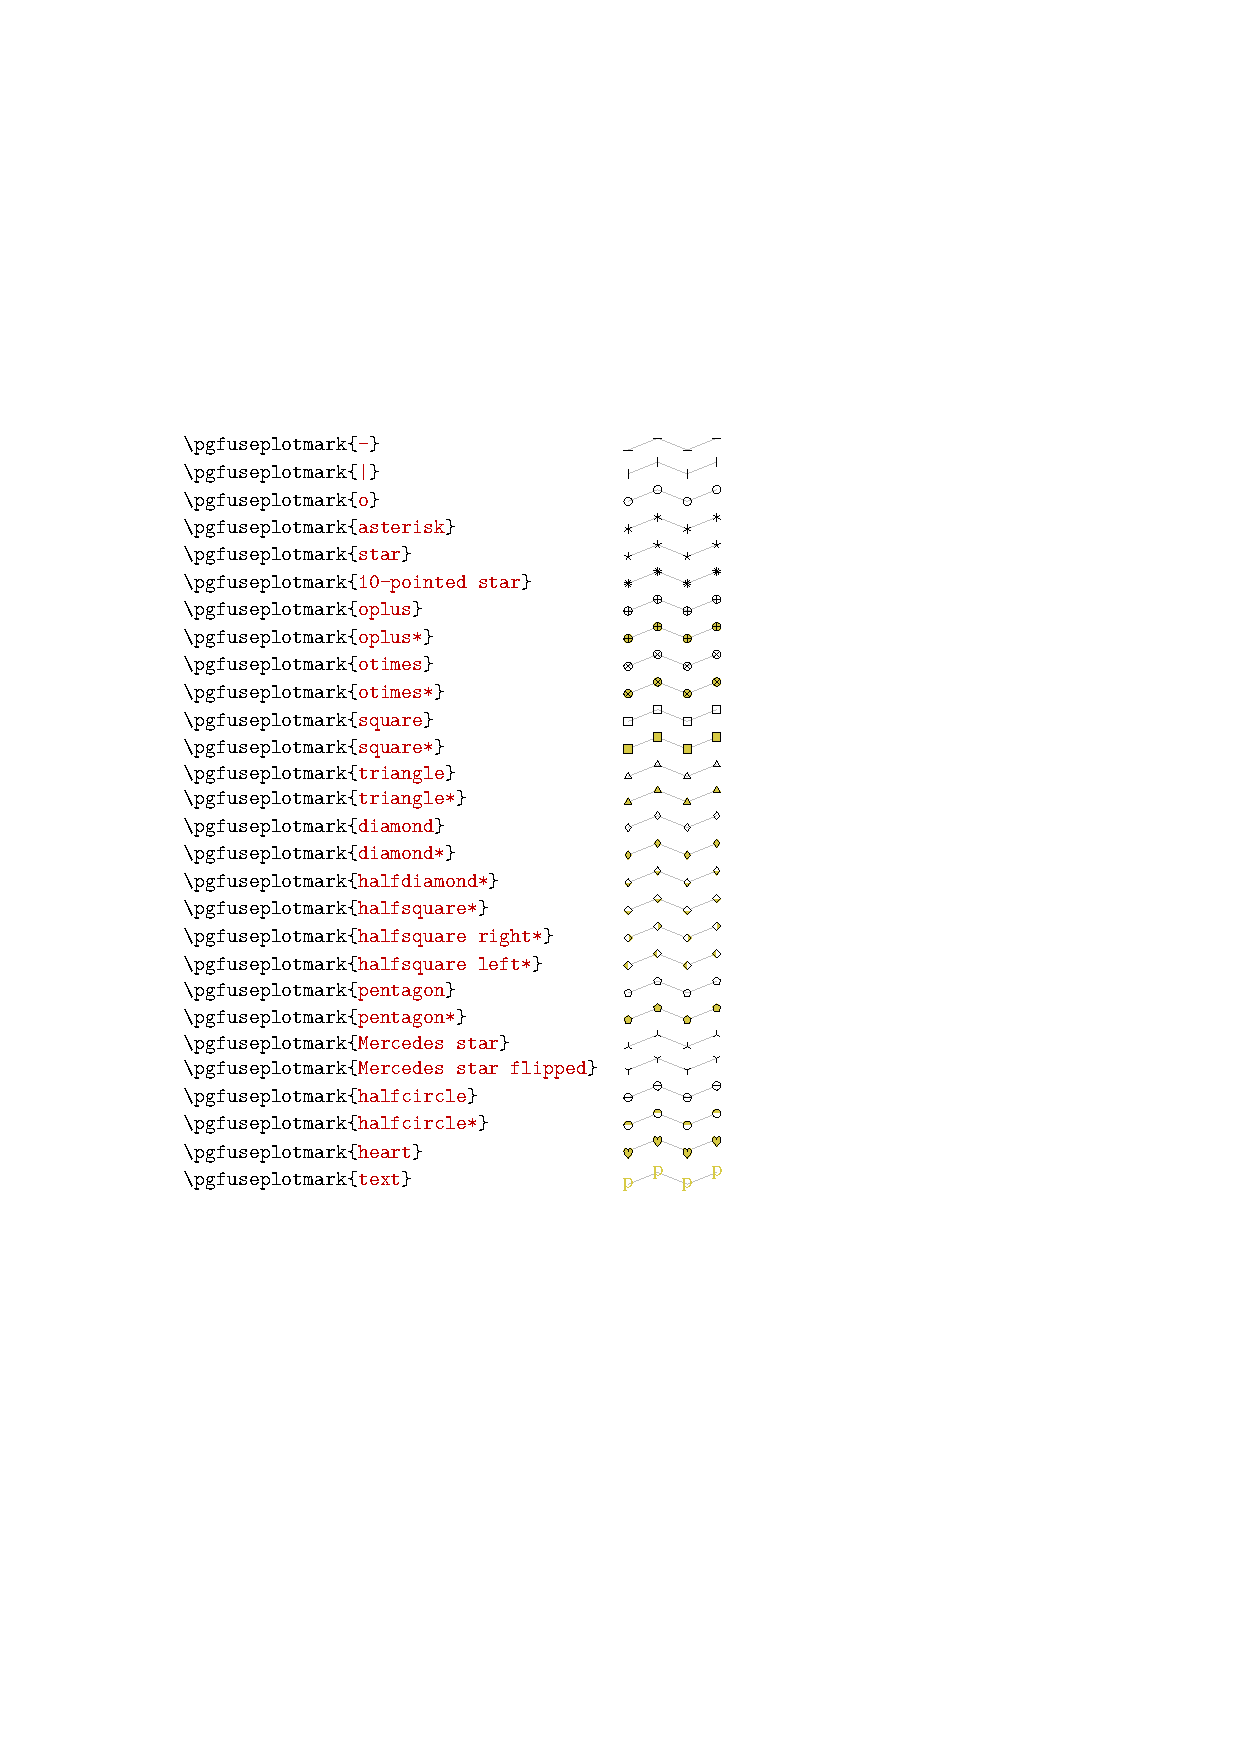
\includegraphics[width=\linewidth]{./support/pics/point_marker.pdf}
  \caption{\TikZ{} Marker Style}
  \label{fig:point-marker}
\end{figure}


\subsection{测试数据/代码}\label{imple:code-data}
\def\exampleUR{\textcolor{red}{\sffamily sine.data}}
\begin{DocExample}
# Curve 0 of 1, 10 points
# Curve title: "f(x)"
# x y type
-3.14159 -0.00000  i
-2.44346 -0.64279  i
-1.74533 -0.98481  i
-1.04720 -0.86603  i
-0.34907 -0.34202  i
0.34907 0.34202  i
1.04720 0.86603  i
1.74533 0.98481  i
2.44346 0.64279  i
3.14159 0.00000  i
\end{DocExample}


\def\exampleUR{\textcolor{red}{\sffamily table.py}}
\begin{DocExample}[@@]
\begin{pycode}{pycode-1.py}
import numpy as np

# write file
with open ('./ztikz_output/python_data/pycode-1.py.out', 'w') as file:
  file.write("\\begin{tabular}{p{3cm}ccc}\n")
  file.write("\\hline\n")
  file.write("number/function & $\\sin$ & $\\cos$ & $\\tan$\\\\\n")
  file.write("\\hline\n")
  for i in range(1, 16):
    file.write(
      f"${i}$ & ${np.around(np.sin(i), decimals=4)}$ &  ${np.around(np.cos(i), decimals=4)}$ & ${np.around(np.tan(i), decimals=4)}$\\\\\n"
    )

  file.write("\\hline\n")
  file.write("\\end{tabular}\n")
\end{pycode}
\end{DocExample}


\clearpage
\section{TODO}
\ztikz{} 的开发暂且告一段落了, 这里列出部分将来可能会增加的功能
(\undone{} -- 未完成; \done{} -- 已完成; \wontfix{} -- 不考虑该功能):


\let\olditem\item
\RenewDocumentCommand{\item}{so}
  {
    \IfValueTF{#2}
      {\color{black}\def\checkmark{\IfBooleanTF{#1}{\wontfix}{\done}}% 
        \olditem\IfBooleanTF{#1}{(#2)}{\IfValueT{#2}{#2-}已完成:}\color{gray}}
      {\color{black}\def\checkmark{\IfBooleanTF{#1}{\wontfix}{\undone}}%
        \olditem}
  }
\begin{todolist}
  \item 实现类似 \pkg{tikz-3dplot} 的接口, 使用 \LaTeX3 对其进行重写.
  \item 增加 Matlab 脚本的调用接口, 或者直接使用其开源替代 \href{https://octave.org/}{GNU Octave} ?
  \item 实现 \env{wolframAny} 环境, 该环境实现的功能类似 \env{pycode}.
  \item 重写缓存机制对应的函数 \cs{ztikz_hash_if_change:nn}, 目前不够灵活(或许直接使用 \href{https://github.com/leo-colisson/robust-externalize}{\pkg{robust-externalize}} 宏包).
  \item 针对 \pkg{cache} 库, 需要清除多余的 Hash 值: 例如某个环境/命令产生的原 Hash 值为 ``A'', 对应环境/命令中的参数改变后,其 Hash 值变为了 ``B'', 那么此时需要清除原始的 ``A''.
\end{todolist}


% ----------------------------------------------------------------------
%                              Implement
% ----------------------------------------------------------------------
\newgeometry{left=1in, top=0pt, right=.9in, bottom=0pt}
\ztexDocPrintSource


\newgeometry{left=1in, top=.75in, right=.9in, bottom=.75in}
\renewcommand\indexname{索引}
\PrintIndex
\end{document}